\documentclass[a4paper]{article}

% Basic packages
\usepackage{fontspec}
\XeTeXlinebreaklocale "zh"    % 启用中文断行（XeTeX 内建，无需 xeCJK）
\XeTeXlinebreakskip = 0pt plus 1pt
\setmainfont{Songti SC}
\setsansfont{Heiti SC}
\setmonofont{Menlo}
\usepackage{amsmath, amssymb}
\usepackage{graphicx}
\usepackage[margin=2.5cm]{geometry}
\usepackage[most]{tcolorbox}
\usepackage{etoolbox}
\usepackage{listings}
\usepackage{hyperref}
\usepackage{booktabs}
\usepackage{subcaption}
\usepackage{float}

% Chinese font setup (macOS system fonts, no ctex needed)
\setmainfont{Songti SC}
\setsansfont{Heiti SC}
\setmonofont{Menlo}
\newcommand{\song}{\fontspec{Songti SC}}
\newcommand{\hei}{\fontspec{Heiti SC}}
\newcommand{\kai}{\fontspec{KaiTi}}
\newcommand{\fangsong}{\fontspec{FangSong}}

% ===== Highlight boxes =====
\newtcolorbox{knowledgebox}[1]{
    enhanced, colback=blue!5!white, colframe=blue!75!black, colbacktitle=blue!75!black,
    coltitle=white, fonttitle=\bfseries, title=#1, attach boxed title to top left={yshift=-2mm, xshift=2mm},
    boxrule=1pt, sharp corners
}

\newtcolorbox{importantbox}[1]{
    enhanced, colback=yellow!10!white, colframe=yellow!80!black, colbacktitle=yellow!80!black,
    coltitle=black, fonttitle=\bfseries, title=#1, sharp corners
}

\newtcolorbox{warningbox}[1]{
    enhanced, colback=red!5!white, colframe=red!75!black, colbacktitle=red!75!black,
    coltitle=white, fonttitle=\bfseries, title=#1, sharp corners
}

\newtcolorbox{practicebox}[1]{
    enhanced, colback=green!5!white, colframe=green!60!black, colbacktitle=green!60!black,
    coltitle=white, fonttitle=\bfseries, title=#1, sharp corners
}

% ===== Code listings =====
\lstset{
    basicstyle=\ttfamily\small,
    keywordstyle=\color{blue},
    stringstyle=\color{red!60!black},
    commentstyle=\color{green!60!black},
    breaklines=true,
    frame=single,
    numbers=left,
    numberstyle=\tiny\color{gray},
    captionpos=b,
    extendedchars=false
}

% ===== Front-page metadata =====
\newcommand{\notetitle}{CS336 Lecture 17：对齐——强化学习（下）}
\newcommand{\notesubtitle}{Stanford CS336: Language Modeling from Scratch (Spring 2025)}
\newcommand{\noteauthors}{讲师：Percy Liang \quad 笔记：ZCode}
\newcommand{\notedate}{2026-07-14}
\newcommand{\videochannel}{Stanford CS336}
\newcommand{\videopublishdate}{2025 Spring}
\newcommand{\videoduration}{76 分钟}
\newcommand{\videourl}{https://www.youtube.com/watch?v=JdGFdViaOJk}
\newcommand{\videocoverpath}{cover.jpg}

\begin{document}

% ===== Title page =====
\begin{titlepage}
\centering
{\Large 课程笔记\par}
\vspace{1.2cm}
{\huge\bfseries \notetitle\par}
\vspace{0.3cm}
{\large \notesubtitle\par}
\vspace{0.5cm}
{\large \noteauthors\par}
\vspace{0.3cm}
{\large \notedate\par}
\vspace{1.0cm}

\includegraphics[width=0.82\textwidth,height=0.40\textheight,keepaspectratio]{\videocoverpath}\par

\vfill
\begin{tcolorbox}[width=0.9\textwidth, colback=black!2!white, colframe=black!60, sharp corners]
\textbf{视频作者/频道}：\videochannel\par
\textbf{发布日期}：\videopublishdate\par
\textbf{视频时长}：\videoduration\par
\textbf{视频链接}：\href{\videourl}{\nolinkurl{\videourl}}
\end{tcolorbox}
\end{titlepage}

\tableofcontents
\newpage

%% --- 正文内容开始 ---

\section{导言：本讲的定位}

这是课程的最后一堂主讲课。Percy Liang 开篇就定位了本讲的性质：上一堂课 Tatsu 给出了"带验证器奖励的强化学习"（RL from verifiable rewards）的总览，介绍了 PPO、GRPO 等策略梯度算法的概念。本讲\textbf{不引入新内容}，而是对策略梯度（特别是 GRPO）的\textbf{机制做深度拆解}——把抽象的算法落到代码与数学上，并配套一个可以在笔记本上跑通的玩具任务。

\begin{importantbox}{本讲的三条主线}
\begin{enumerate}
\item \textbf{建立形式化}：把语言模型的 RL 设置（状态、动作、奖励、转移动力学）讲精确。
\item \textbf{方差与基线}：为什么朴素策略梯度噪声大，基线（baseline）/优势函数（advantage）如何降低方差。
\item \textbf{GRPO 全流程代码}：用一个"排序"玩具任务和极简模型，逐块讲清 rollout、reward、delta、log-prob、clipped loss、KL 惩罚与训练循环。
\end{enumerate}
\end{importantbox}

Percy 特别提醒：GRPO 的\textbf{具体形式不是最重要的}——明年可能就有 GRPO2，但策略梯度的核心数学是稳定的，"明年我还会讲同样的内容"。这一讲的价值在于把"算法菜单"和"取舍直觉"交到学生手里。

\section{语言模型 RL 的形式化设置}

\subsection{状态、动作、奖励}

强化学习的三大要素在语言模型里有非常具体的含义。Percy 强调要把"显而易见"的东西讲清楚。

\begin{figure}[H]
\centering
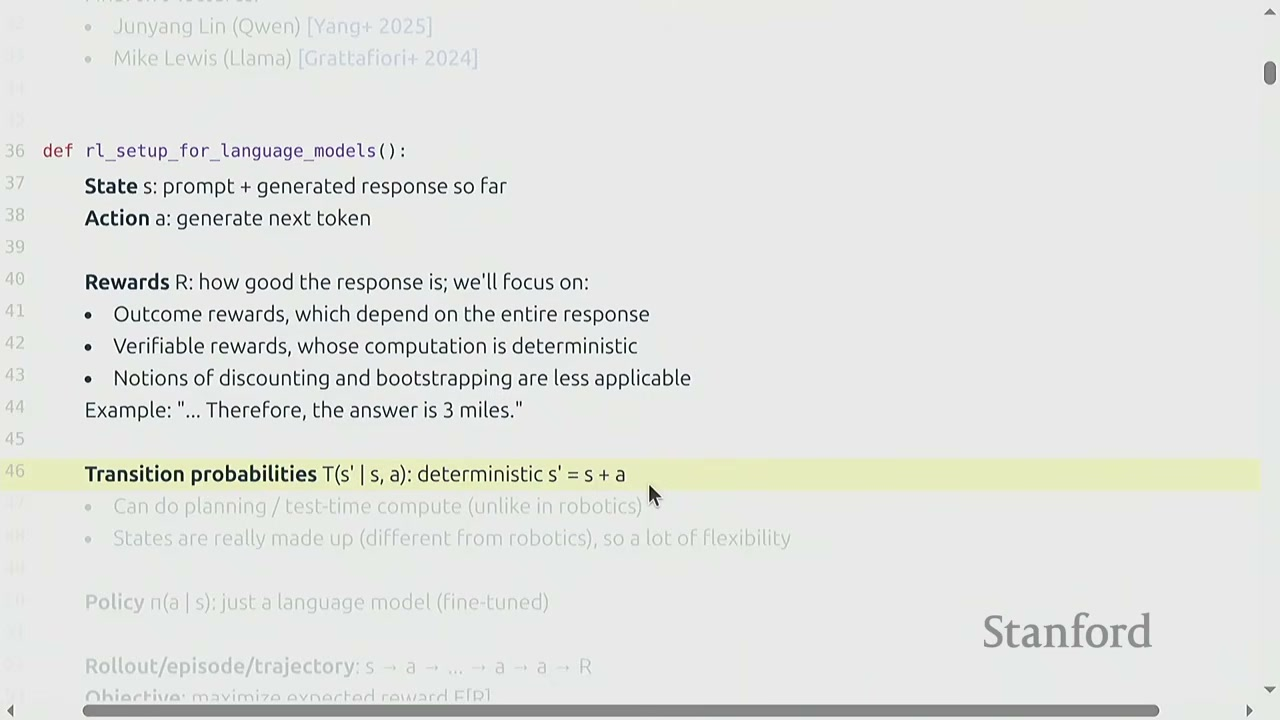
\includegraphics[width=\textwidth]{figures/fig_01_rl_setup.jpg}
\caption{语言模型 RL 的设置：状态 = prompt + 已生成响应；动作 = 下一个 token；奖励 = 响应的好坏\protect\footnotemark}
\end{figure}
\footnotetext{视频画面时间区间：00:02:45--00:03:30。}

\begin{tabular}{p{2.5cm}p{11cm}}
\toprule
\textbf{要素} & \textbf{在语言模型中的含义} \\
\midrule
状态 $s$ & prompt 加上到目前为止生成的响应（即已写出的 token 序列） \\
动作 $a$ & 生成下一个 token \\
策略 $\pi_\theta(a \mid s)$ & 语言模型本身，给定上文输出下一 token 分布 \\
奖励 $r$ & 整个响应有多好；本课聚焦\textbf{结果奖励（outcome reward）} \\
\bottomrule
\end{tabular}

本课的两个核心假设：

\begin{itemize}
\item \textbf{结果奖励}：奖励是整个响应的函数，不是中间每一步都有奖励。
\item \textbf{可验证奖励}：奖励计算是确定性的——某个函数直接返回数值（如对答案），而不需要问人。这与 RLHF 中需要从偏好数据估计的奖励模型不同。
\end{itemize}

\begin{figure}[H]
\centering
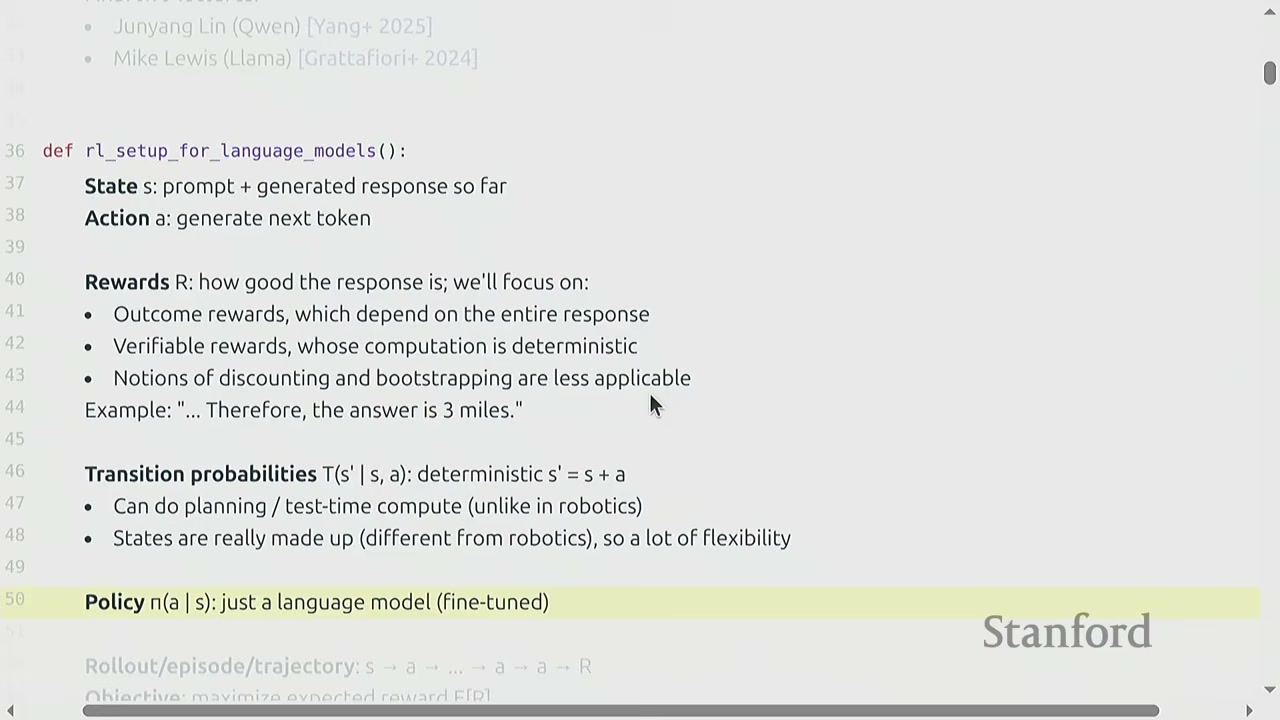
\includegraphics[width=\textwidth]{figures/fig_02_outcome_reward.jpg}
\caption{结果奖励的典型形态：数学题里模型生成一段思维链，最后输出"答案是 3 英里"，奖励函数提取答案并与 ground truth 比对\protect\footnotemark}
\end{figure}
\footnotetext{视频画面时间区间：00:04:30--00:05:15。}

\begin{warningbox}{稀疏与延迟奖励}
整条轨迹只在最后得到一个奖励信号。这带来了\textbf{稀疏（sparse）}与\textbf{延迟（delayed）}两大难题：如果策略太差、rollout 全错，梯度近似为零，模型就"卡住"了。但也正因为如此，概念上更简单——不必处理折扣（discounting）和 bootstrapping。
\end{warningbox}

\subsection{转移动力学与"可规划性"}

\begin{figure}[H]
\centering
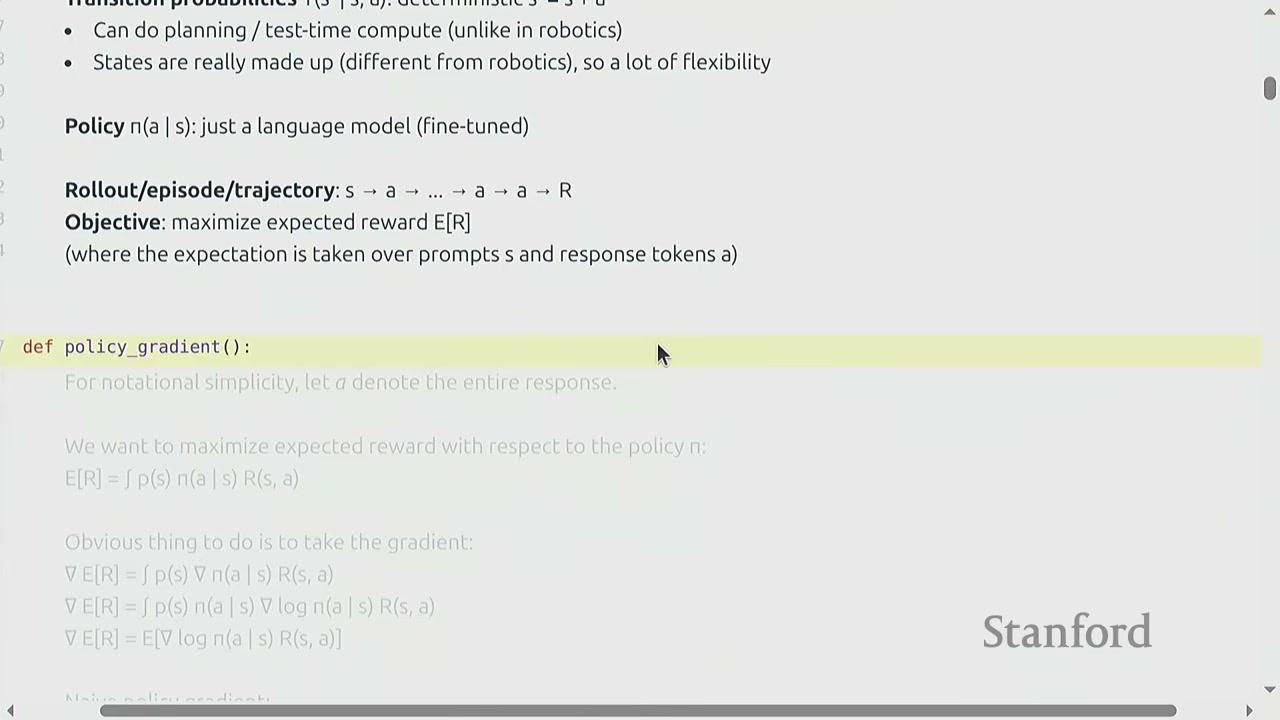
\includegraphics[width=\textwidth]{figures/fig_03_transition_dynamics.jpg}
\caption{转移动力学极简：新状态 = 旧状态拼接新 token；因为动力学已知，可以做规划（test-time compute）\protect\footnotemark}
\end{figure}
\footnotetext{视频画面时间区间：00:05:30--00:06:15。}

在语言模型设定里，\textbf{转移动力学}异常简单：

\[
s_{t+1} = s_t \oplus a_t
\]

也就是把新 token 直接拼到当前序列后面。这有两个深远含义：

\begin{importantbox}{为什么语言模型 RL 与机器人 RL 不同}
\begin{enumerate}
\item \textbf{可以规划}：因为你知道世界动力学，可以模拟未来、做 test-time compute（搜索/采样）。机器人学家做梦都想有这种能力。
\item \textbf{状态是"造出来"的}：状态不是物理量（关节角、图像），而是模型自己生成的 token。因此模型可以自由构造自己的 scratchpad（思维链）来推导答案。难点不是"能否到达某状态"（写什么 token 都行），而是\textbf{这些 token 是否真的导向正确答案}。
\end{enumerate}
\end{importantbox}

这种"状态自由"是把双刃剑：它解锁了思维链与自我改进，但也让信用分配（credit assignment）更难——你不知道是早期决策重要还是结尾重要。

\subsection{策略与目标函数}

\begin{figure}[H]
\centering
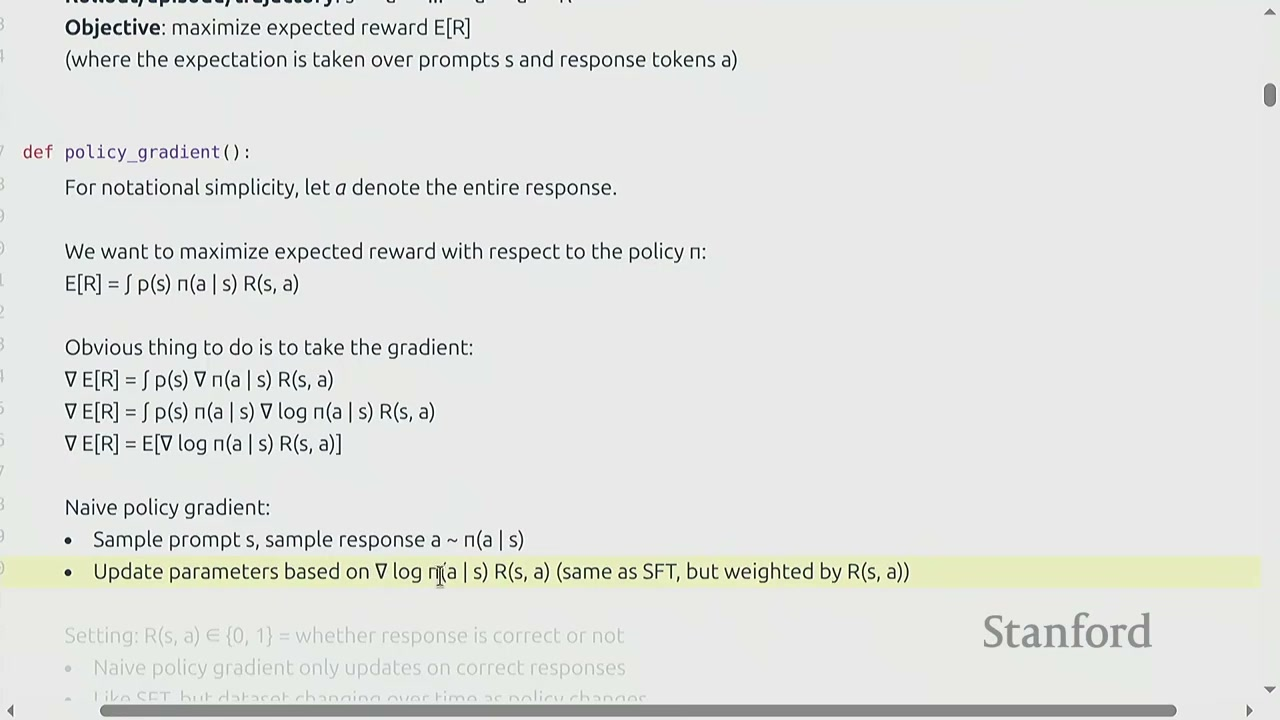
\includegraphics[width=\textwidth]{figures/fig_04_policy_objective.jpg}
\caption{策略即语言模型；目标是最大化期望奖励，期望同时遍历 prompt 分布与策略采样\protect\footnotemark}
\end{figure}
\footnotetext{视频画面时间区间：00:07:45--00:08:30。}

策略 $\pi_\theta$ 通常由一个预训练语言模型微调而来。整条从 prompt 到响应的过程也叫 rollout / episode / trajectory。形式化目标为：

\[
J(\theta) = \mathbb{E}_{s \sim p(s),\; a \sim \pi_\theta(\cdot \mid s)}\left[ r(s, a) \right]
\]

\begin{itemize}
\item $p(s)$：环境给出的 prompt 分布
\item $\pi_\theta(\cdot \mid s)$：当前策略对响应的采样分布
\item $r(s, a)$：结果奖励
\end{itemize}

为简化记号，后续用 $a$ 直接表示\textbf{整条响应}（而非单个 token），因为结果奖励下这与"一次生成所有动作"等价。

\section{策略梯度：从目标到更新}

\subsection{策略梯度定理}

\begin{figure}[H]
\centering
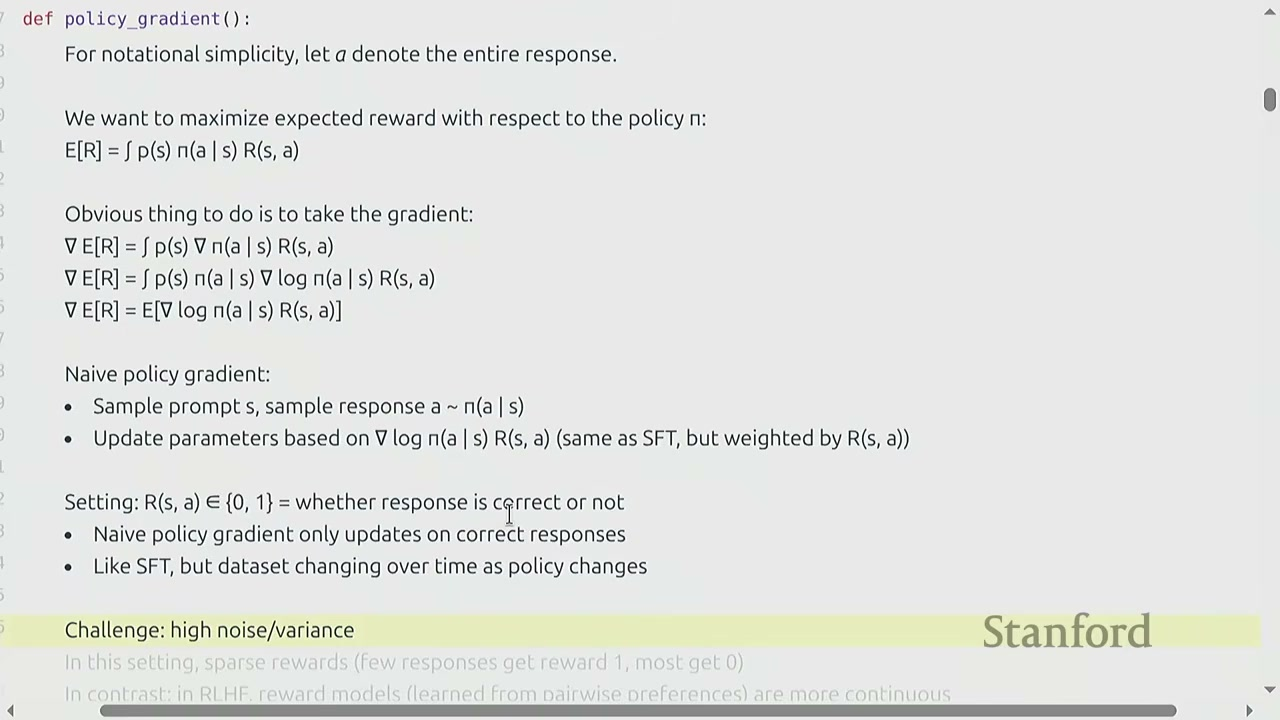
\includegraphics[width=\textwidth]{figures/fig_05_pg_theorem.jpg}
\caption{策略梯度推导：对期望奖励求梯度，梯度只作用于策略；用 $\nabla \log$ 的链式法则改写为可采样估计\protect\footnotemark}
\end{figure}
\footnotetext{视频画面时间区间：00:09:00--00:09:45。}

策略梯度的核心是把"对期望求导"转化为"可采样的估计"。对 $J(\theta) = \int p(s)\,\pi_\theta(a\mid s)\,r(s,a)\,ds\,da$ 求梯度，梯度只触碰策略项：

\[
\nabla_\theta J(\theta) = \mathbb{E}_{s,a}\left[ r(s,a)\,\nabla_\theta \log \pi_\theta(a \mid s) \right]
\]

\begin{knowledgebox}{为什么能这样换？}
关键恒等式 $\nabla \log \pi = \nabla \pi / \pi$（即 $\nabla \pi = \pi \cdot \nabla \log \pi$）。把它代回积分，多出的 $\pi$ 把期望"还原"回来。这就是"策略梯度定理"，本质就是\textbf{对数导数技巧（log-derivative trick）}。
\end{knowledgebox}

\subsection{朴素策略梯度及其 SFT 类比}

\begin{figure}[H]
\centering
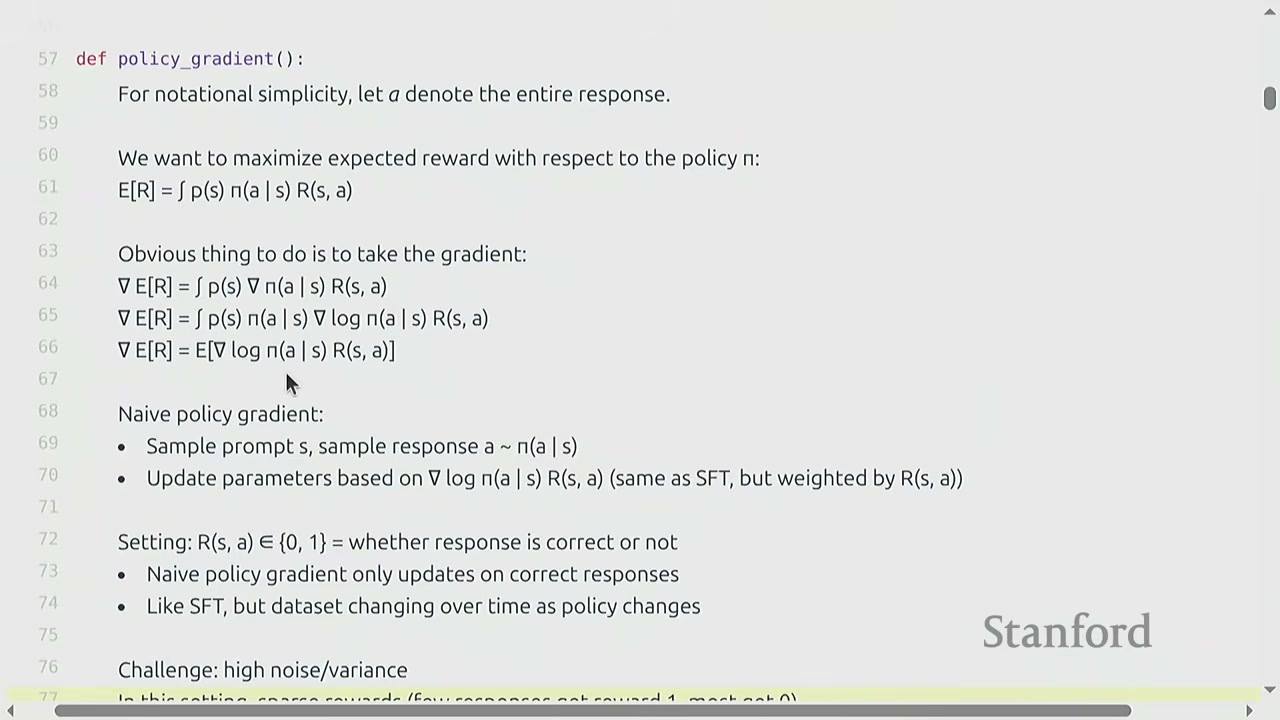
\includegraphics[width=\textwidth]{figures/fig_06_naive_pg_sft.jpg}
\caption{朴素策略梯度 = 带 reward 加权的 SFT：采样一个 prompt、采样一个响应、按 $r \cdot \nabla\log\pi$ 更新\protect\footnotemark}
\end{figure}
\footnotetext{视频画面时间区间：00:10:45--00:11:30。}

朴素策略梯度就是 SGD 的直接套用：

\[
\theta \leftarrow \theta + \eta \cdot r(s,a)\,\nabla_\theta \log \pi_\theta(a \mid s)
\]

\begin{importantbox}{与 SFT 的深刻类比}
SFT 是人写出 $a$，模型模仿 $a$、最大化其概率。朴素策略梯度里 $a$ 由模型自己生成，但\textbf{整体被 reward 加权}。若 reward 是 $\{0,1\}$：

\begin{itemize}
\item $r=1$（答对）：等价于在该响应上做 SFT，提升概率。
\item $r=0$（答错）：梯度为零，完全忽略。
\end{itemize}

唯一区别是\textbf{数据集随时间变化}：每次更新后策略变了，重新采样的数据集分布也变了（且希望越来越好）。
\end{importantbox}

\subsection{高方差与稀疏奖励陷阱}

\begin{figure}[H]
\centering
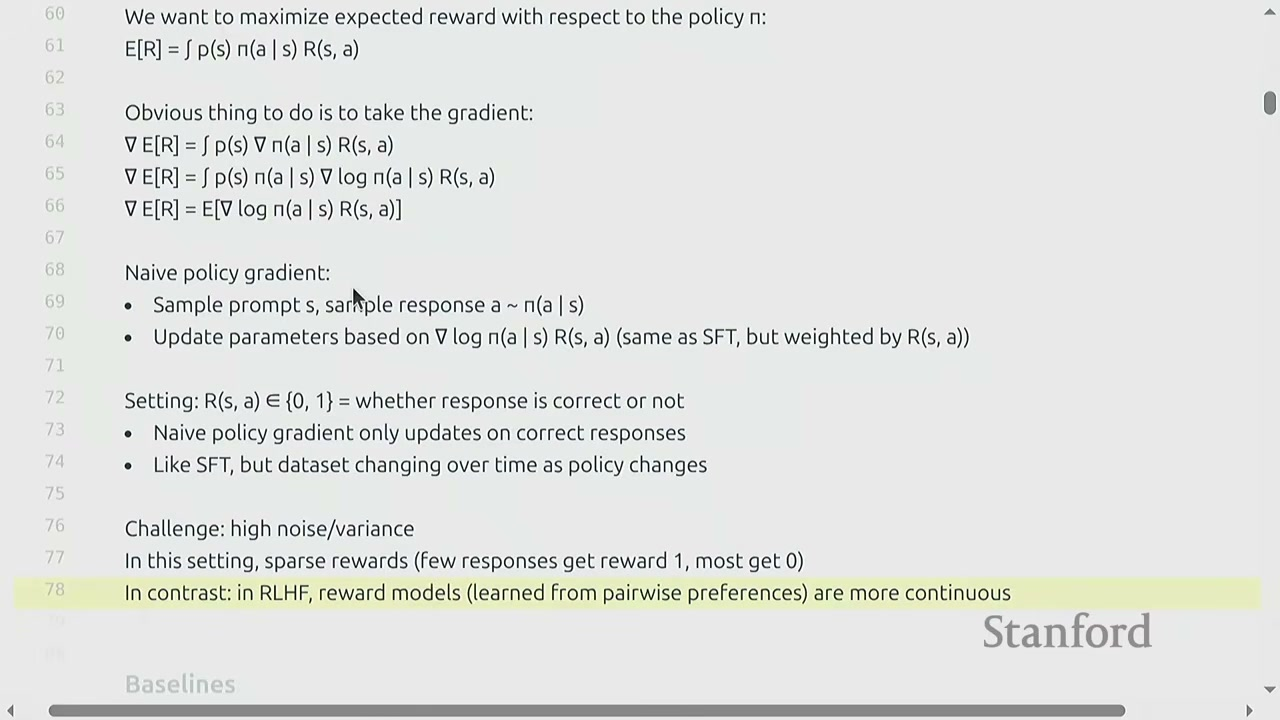
\includegraphics[width=\textwidth]{figures/fig_07_sparse_reward.jpg}
\caption{稀疏奖励陷阱：策略太差时 rollout 全错，$r=0$，梯度为零，模型卡死；与 RLHF 的连续 reward 形成对比\protect\footnotemark}
\end{figure}
\footnotetext{视频画面时间区间：00:12:15--00:13:00。}

监督学习的 SGD 也会有噪声，但 RL 是"另一个量级"的噪声。在 $\{0,1\}$ 奖励的稀疏设定下：

\begin{warningbox}{卡死问题}
如果策略太差，几乎所有 rollout 都得 $r=0$，梯度近似为零，参数不动。\textbf{监督学习至少保证每步都朝某方向更新，而 RL 不保证}。这正是为什么需要基线/奖励塑形/partial credit 等技巧。

唯一出路：只要偶尔能蒙对几道简单题拿到 reward，就能更新、泛化，下一轮采样到略难的题也能做对——数据集 reward 单调上升。
\end{warningbox}

Percy 回答了一个好问题："为什么不把 $0$ 改成 $-1$？"——他指出这会被基线机制\textbf{自动}处理：用 reward 减去均值后，原来全 $0$ 的 batch 也会出现负的 advantage，从而对错答施加"推远"的更新。

\section{方差、基线与优势函数}

\subsection{两状态玩具例子：理解高方差}

\begin{figure}[H]
\centering
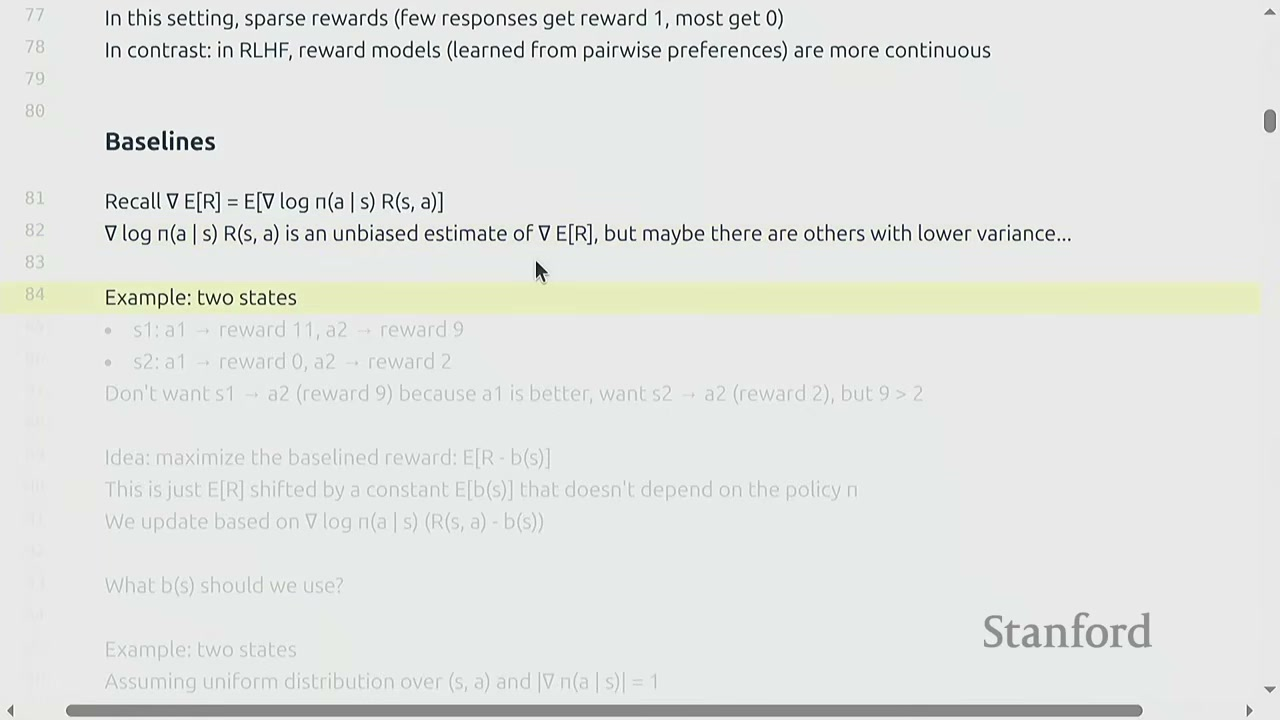
\includegraphics[width=\textwidth]{figures/fig_08_two_state_variance.jpg}
\caption{两状态例子：$S_1$（简单题）的次优动作也拿 reward 9，比 $S_2$（难题）的最优动作（reward 2）还高，朴素梯度会被误导\protect\footnotemark}
\end{figure}
\footnotetext{视频画面时间区间：00:16:15--00:17:00。}

Percy 给了一个具象例子来展示"高方差"到底是什么。设两状态 $S_1$（易）、$S_2$（难），各有两动作：

\begin{tabular}{p{2cm}p{3cm}p{3cm}p{4cm}}
\toprule
状态 & 动作 A1 reward & 动作 A2 reward & 最优策略 \\
\midrule
$S_1$（易题） & 11 & 9 & 选 A1 \\
$S_2$（难题） & 0 & 2 & 选 A2 \\
\bottomrule
\end{tabular}

\begin{warningbox}{被误导的局部信号}
朴素梯度只看绝对 reward。若在 $S_1$ 上选了次优 A2 拿到 9，会得到"很大的正向梯度"；而在 $S_2$ 上选最优 A2 只拿 2，梯度小。于是模型拼命强化 $S_1 \to A2$，把概率质量从真正的最优 $A1$ 上挤走，陷入局部最优。整体期望上数学终究是对的，但需要"看到全貌"才成立——单步采样的噪声正是源于此。
\end{warningbox}

\subsection{基线的思想}

\begin{figure}[H]
\centering
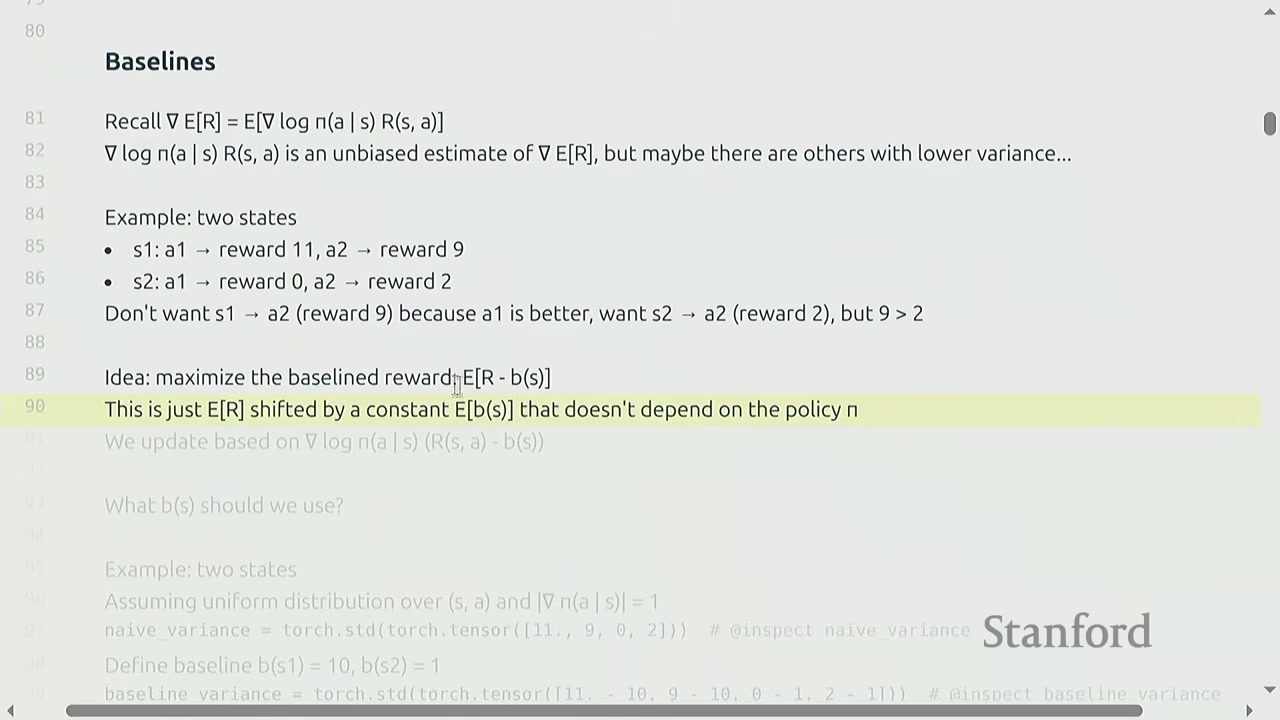
\includegraphics[width=\textwidth]{figures/fig_09_baseline_idea.jpg}
\caption{基线思想：从 reward 减去一个只依赖 $s$ 的函数 $B(s)$，不改变优化问题（期望为常数），但能降方差\protect\footnotemark}
\end{figure}
\footnotetext{视频画面时间区间：00:19:30--00:20:15。}

核心技巧：用 $r - B(s)$ 替换 $r$，其中 $B$ 只依赖状态、不依赖动作。

\[
\nabla_\theta J(\theta) = \mathbb{E}_{s,a}\left[ \big(r(s,a) - B(s)\big)\,\nabla_\theta \log \pi_\theta(a \mid s) \right]
\]

\begin{importantbox}{为什么减基线不改变梯度？}
因为 $\mathbb{E}_{a \sim \pi(\cdot\mid s)}[\nabla_\theta \log \pi_\theta(a\mid s)] = \int \pi \cdot \frac{\nabla \pi}{\pi}\,da = \nabla_\theta \int \pi\,da = \nabla_\theta 1 = 0$。所以 $B(s)$ 项的期望贡献为零，\textbf{梯度不变，只是估计的方差变了}。这对任何不依赖 $a$ 的 $B(s)$ 都成立。
\end{importantbox}

\subsection{基线如何降方差：回到例子}

\begin{figure}[H]
\centering
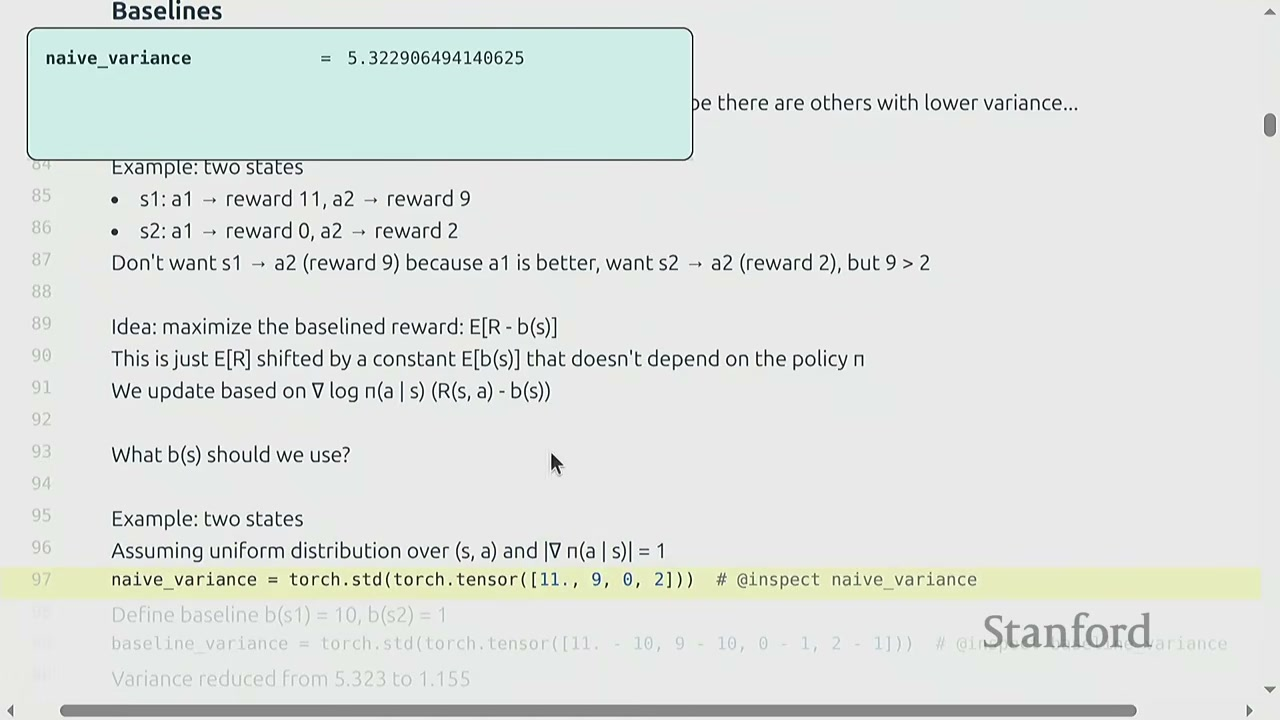
\includegraphics[width=\textwidth]{figures/fig_10_baseline_variance.jpg}
\caption{同一例子加基线后：方差从 5.3 降到 1.1；降低方差意味着更快收敛\protect\footnotemark}
\end{figure}
\footnotetext{视频画面时间区间：00:21:15--00:22:00。}

回到两状态例子。设初始策略均匀、梯度模长为 1。原始 reward 取值 $\{11,9,0,2\}$，方差为 5.3。取基线 $B(S_1)=10$、$B(S_2)=1$（即各状态的"平均 reward"），则 advantage 为：

\[
S_1:\; 11-10=1,\; 9-10=-1; \qquad S_2:\; 0-1=-1,\; 2-1=1
\]

\begin{itemize}
\item 现在每个状态的"次优动作" advantage 为负，会被\textbf{推远}；最优动作 advantage 为正，会被\textbf{拉近}。
\item 方差降到 1.1。降方差直接意味着更快收敛。
\end{itemize}

\begin{knowledgebox}{$B(s)$ 与"冻结策略"的关系}
$B(s)$ 不能依赖当前可训练策略 $\pi_\theta$。但你可以\textbf{冻结}某个旧策略当常数用——只要不对其求导。实操中通常保留一个 old/reference 副本，更新若干步后再同步。PPO 用 value function 充当这个角色。
\end{knowledgebox}

\subsection{最优基线与启发式选择}

\begin{figure}[H]
\centering
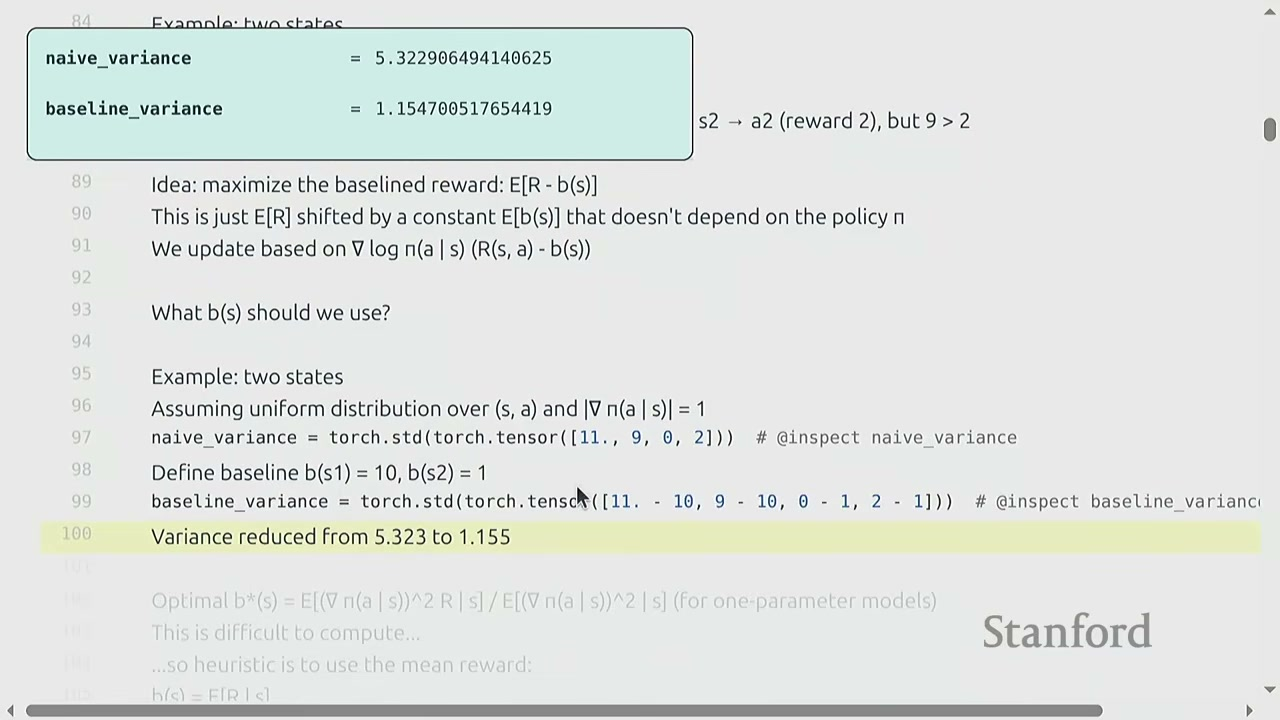
\includegraphics[width=\textwidth]{figures/fig_11_optimal_baseline.jpg}
\caption{最优基线有闭式解但难以计算（涉及协方差）；实践中常用启发式 $B(s) \approx \mathbb{E}[r \mid s]$（即 value function）\protect\footnotemark}
\end{figure}
\footnotetext{视频画面时间区间：00:24:15--00:25:00。}

对单参数模型，最优基线有闭式解：

\[
B^*(s) = \frac{\mathbb{E}_a\left[ \|\nabla_\theta \log \pi_\theta(a\mid s)\|^2 \, r(s,a) \right]}{\mathbb{E}_a\left[ \|\nabla_\theta \log \pi_\theta(a\mid s)\|^2 \right]}
\]

\begin{itemize}
\item 多维情形下分子分母会变成协方差结构，\textbf{计算昂贵}。
\item 实践中通常忽略梯度模长权重，退化为启发式：$B(s) \approx \mathbb{E}_{a}[r \mid s]$，即给定 prompt 的期望 reward（这就是 value function $V(s)$ 的定义）。
\item 即使这个期望也算不出来，只能估计——但它给出了"基线应该长什么样"的指导原则。
\end{itemize}

\subsection{优势函数}

\begin{figure}[H]
\centering
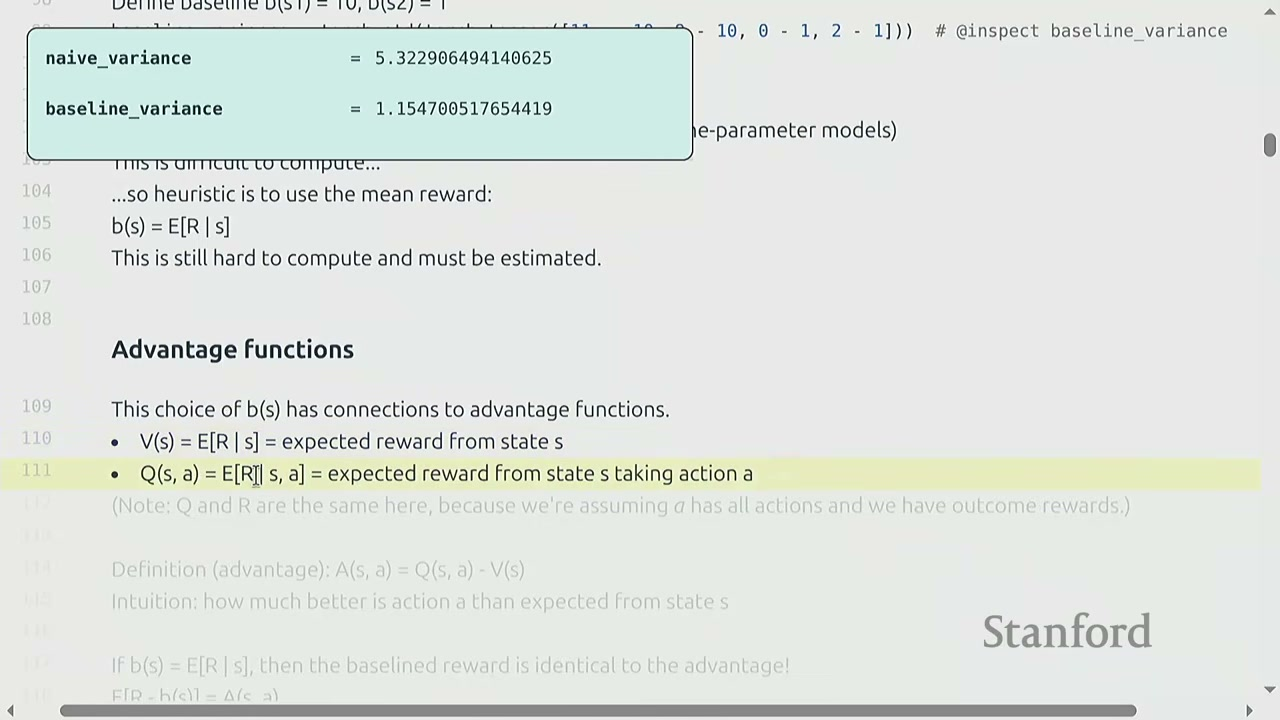
\includegraphics[width=\textwidth]{figures/fig_12_advantage.jpg}
\caption{Value / Q / Advantage 的定义：$A(s,a) = Q(s,a) - V(s)$，衡量动作 $a$ 比平均水平好多少\protect\footnotemark}
\end{figure}
\footnotetext{视频画面时间区间：00:26:30--00:27:15。}

定义三个标准函数：

\[
V(s) = \mathbb{E}_{a}[r \mid s], \qquad Q(s,a) = r(s,a), \qquad A(s,a) = Q(s,a) - V(s)
\]

\begin{itemize}
\item $V(s)$：value function，状态 $s$ 下的期望 reward。
\item $Q(s,a)$：在结果奖励设定下，因为 $a$ 是整条响应，$Q$ 就等于 $r(s,a)$（一般 RL 里 $Q$ 是回报的期望，这里退化为单步 reward）。
\item $A(s,a)$：advantage，动作 $a$ 相对平均水平的优劣。
\end{itemize}

\begin{importantbox}{基线即优势}
若取启发式 $B(s) = V(s) = \mathbb{E}[r \mid s]$，则 $r - B(s) = Q(s,a) - V(s) = A(s,a)$。即\textbf{"reward 减基线"在这个选择下就是优势函数}。这给出了基线的直观解释：你不是在优化绝对 reward，而是在优化"比平均水平好多少"。
\end{importantbox}

\subsection{统一的 delta 形式}

\begin{figure}[H]
\centering
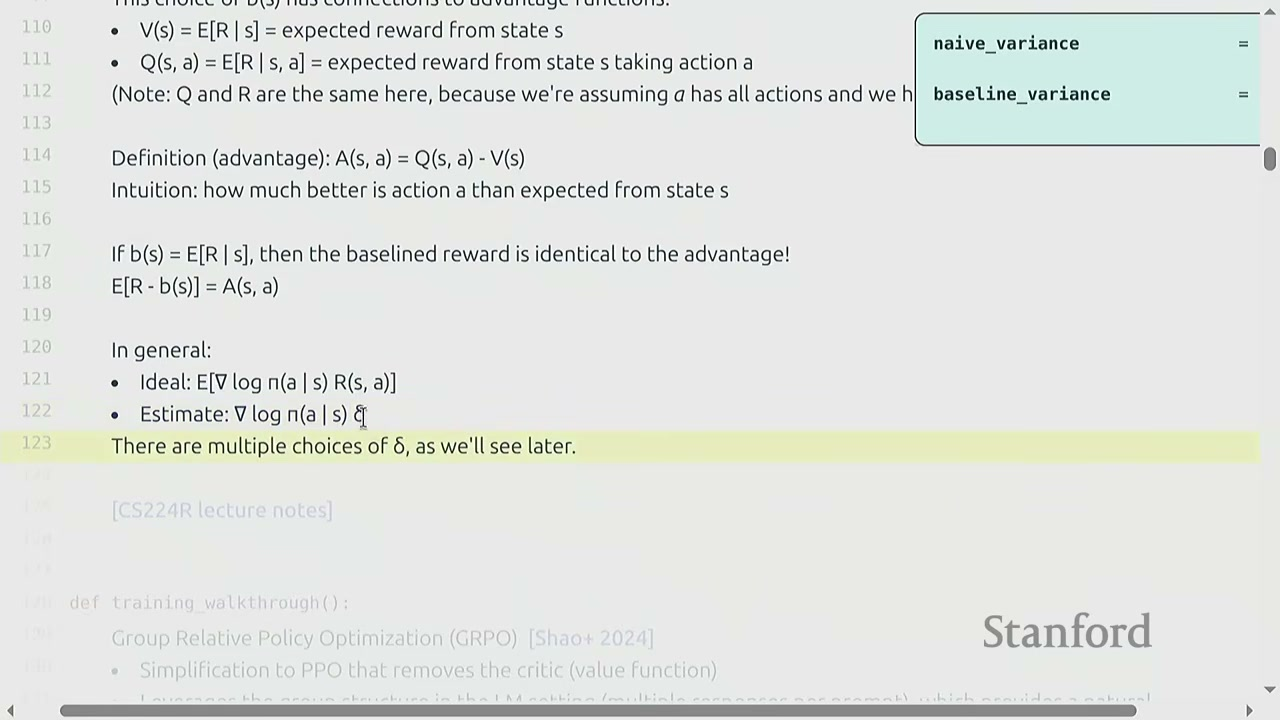
\includegraphics[width=\textwidth]{figures/fig_13_general_delta.jpg}
\caption{所有策略梯度算法统一为 $\nabla \log \pi \cdot \delta$；$\delta$ 的不同选择对应不同算法（reward / 中心化 / 标准化）\protect\footnotemark}
\end{figure}
\footnotetext{视频画面时间区间：00:28:30--00:29:15。}

因为精确算不出这些期望，Percy 用 $\delta$（delta）统一记号——表示放进梯度的那个"东西"：

\[
\nabla_\theta J(\theta) \approx \nabla_\theta \log \pi_\theta(a \mid s) \cdot \delta
\]

\begin{tabular}{p{3.5cm}p{9.5cm}}
\toprule
\textbf{$\delta$ 的选择} & \textbf{对应方法} \\
\midrule
$\delta = r$ & 朴素策略梯度 \\
$\delta = r - \hat{V}(s)$ & 带基线（中心化 reward） \\
$\delta = (r - \hat{V}(s)) / \hat{\sigma}(s)$ & GRPO 式（再除以标准差，尺度不变） \\
\bottomrule
\end{tabular}

\begin{knowledgebox}{算法会变，框架不变}
Percy 反复强调："$\delta$ 的具体形式不是重点——明年会有 GRPO2，但 $\nabla\log\pi \cdot \delta$ 这个框架是永恒的。"这也是为什么本讲花大力气建立这个统一视角。想看更完整的 RL 推导，他推荐 Chelsea Finn 的 Deep RL 课程。
\end{knowledgebox}

\section{GRPO：动机与伪代码}

\subsection{为什么 GRPO 在 2024 年才出现}

\begin{figure}[H]
\centering
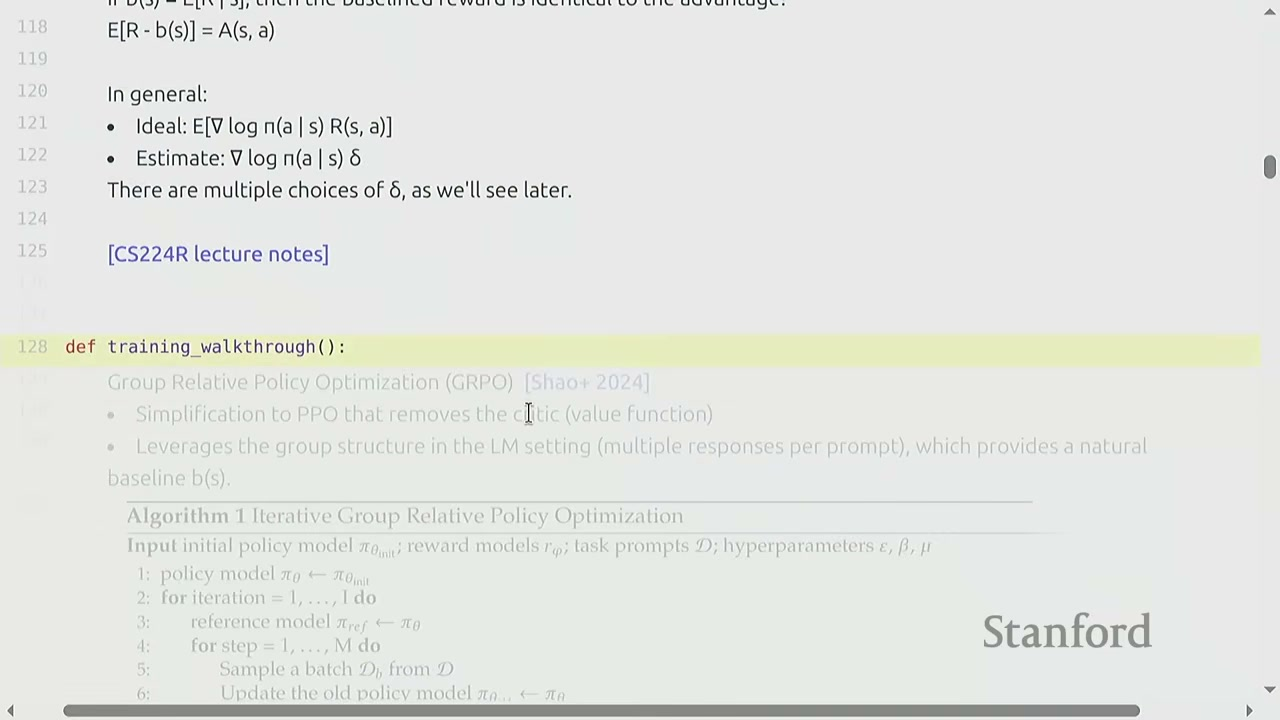
\includegraphics[width=\textwidth]{figures/fig_14_grpo_lineage.jpg}
\caption{GRPO 的谱系：PPO $\to$ DPO $\to$ GRPO；GRPO 是 PPO 的简化，依赖语言模型"一 prompt 多采样"的天然分组结构\protect\footnotemark}
\end{figure}
\footnotetext{视频画面时间区间：00:31:00--00:31:45。}

GRPO 的谱系是 PPO $\to$ DPO $\to$ GRPO。有趣的是，算法往往是"从简单到复杂"演化，但 GRPO 反而是 PPO 的\textbf{简化}。Percy 指出 GRPO 之所以到 2024 年（PPO 是 2017 年）才出现，是因为\textbf{语言模型设定提供了天然的分组结构}：

\begin{importantbox}{GRPO 的核心洞察}
对同一个 prompt 采样多条响应，就得到一个\textbf{自然组（group）}。组内 reward 的均值就是基线 $V(s)$ 的经验估计，组内标准差给出归一化分母。\textbf{组就是天然的对比集合}——GRPO 的 advantage 是"相对组内同伴"的优劣。

经典 RL（机器人走路）每个 rollout 长得都不一样，没有自然分组，只能用 value function 聚合所有可能状态-动作。语言模型的"一 prompt 多采样"让 GRPO 无需 value function。
\end{importantbox}

\subsection{GRPO 伪代码全貌}

\begin{figure}[H]
\centering
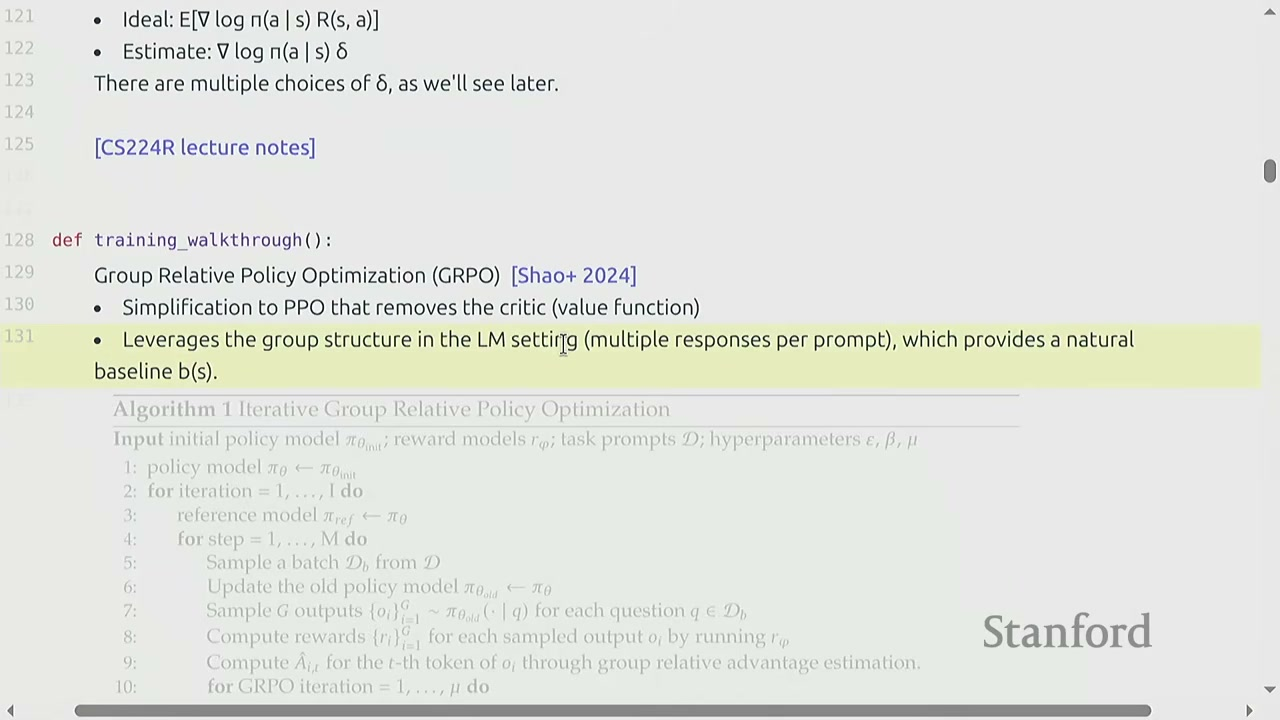
\includegraphics[width=\textwidth]{figures/fig_15_grpo_pseudocode.jpg}
\caption{GRPO 伪代码全貌：rollout $\to$ reward $\to$ delta $\to$ log-prob $\to$ loss $\to$ 梯度步\protect\footnotemark}
\end{figure}
\footnotetext{视频画面时间区间：00:32:30--00:33:15。}

接下来 Percy 把伪代码逐块翻译成可运行 Python。整个流程概括为：

\begin{enumerate}
\item \textbf{生成响应}：给定固定模型，对每个 prompt 采样 $G$ 条响应。
\item \textbf{算 reward}：对每条响应调用奖励函数（与模型无关，除非用 LM-as-judge）。
\item \textbf{算 delta}：根据所选 $\delta$ 变体（原始/中心化/标准化）转换 reward。
\item \textbf{算 log-prob}：把响应过模型，取出每个 token 的对数概率。
\item \textbf{算 loss}：用 log-prob 和 delta 组合（clip 或不 clip），可加 KL 惩罚。
\item \textbf{走梯度步}。
\end{enumerate}

\section{玩具任务：排序与奖励设计}

\subsection{为什么用排序任务}

\begin{figure}[H]
\centering
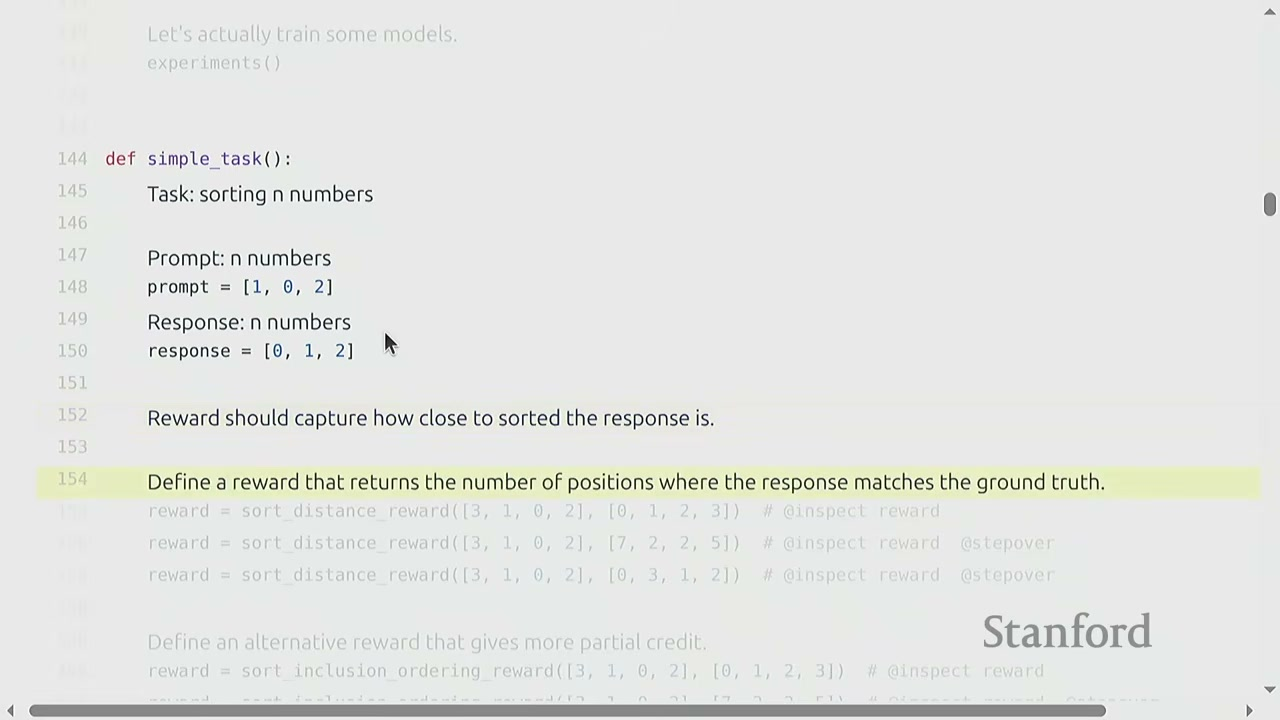
\includegraphics[width=\textwidth]{figures/fig_16_sorting_task.jpg}
\caption{玩具任务：排序 $n$ 个数。Percy 用它是因为可以在笔记本上用极简模型训练，无需 Transformer\protect\footnotemark}
\end{figure}
\footnotetext{视频画面时间区间：00:34:15--00:35:00。}

为了能在没有 GPU 的笔记本上跑通，Percy 设计了一个极简任务：\textbf{排序 $n$ 个数}。prompt 是 $n$ 个数，响应是希望排好序的 $n$ 个数。

\begin{warningbox}{奖励设计是 RL 的艺术}
最直接的奖励是"完全排好序给 1 否则给 0"，但这会触发稀疏 reward 陷阱——策略太差时全得 0，无法更新。因此 Percy 设计了两种给\textbf{部分信用（partial credit）}的奖励。
\end{warningbox}

\subsection{两种奖励函数与部分信用}

\begin{figure}[H]
\centering
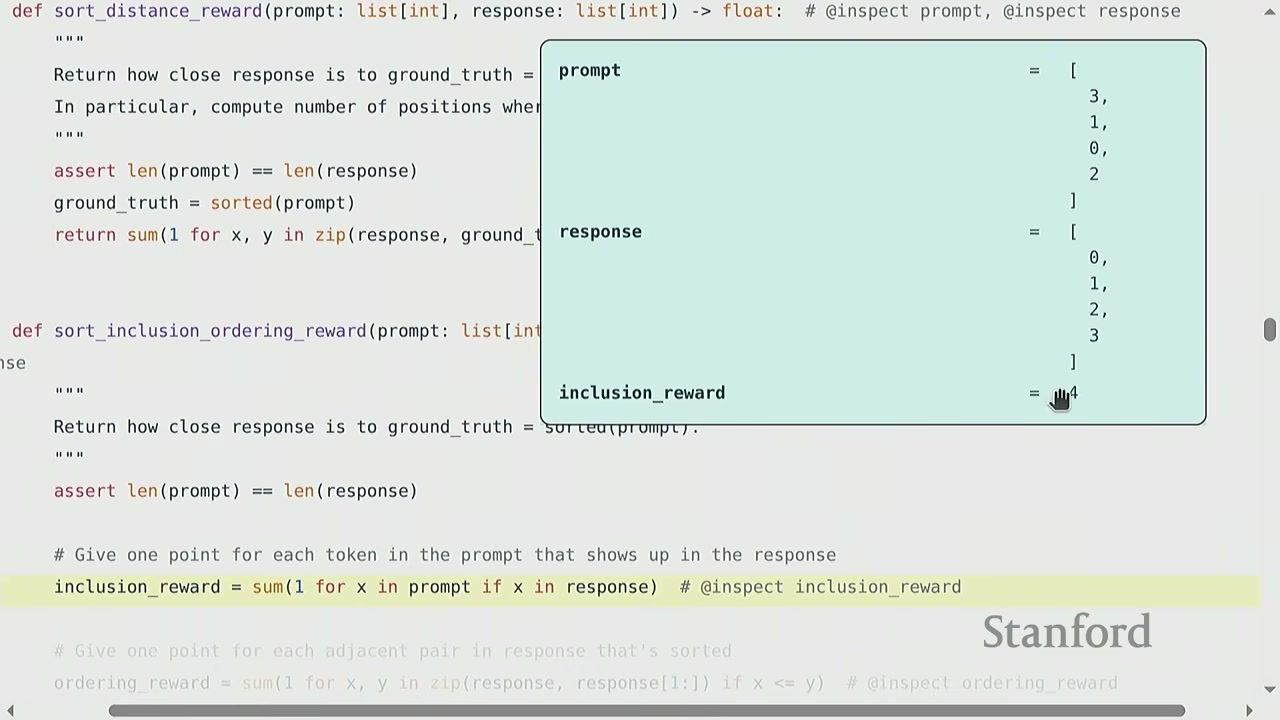
\includegraphics[width=\textwidth]{figures/fig_17_partial_credit.jpg}
\caption{两种部分信用奖励：按位置匹配数；按 inclusion + 相邻对有序数。注意第二种有"漏洞"\protect\footnotemark}
\end{figure}
\footnotetext{视频画面时间区间：00:36:15--00:37:00。}

\textbf{奖励 1（位置匹配）}：响应与 ground truth（即 prompt 的排序）逐位置比对，数匹配的位置数。

\[
r_1 = \sum_{i=1}^{n} \mathbb{1}\big[\text{resp}_i = \text{sorted}(\text{prompt})_i\big]
\]

\textbf{奖励 2（inclusion + 相邻有序）}：每个出现在响应里的 prompt token 得 1 分（鼓励至少输出对的 token）；每个相邻对有序再得 1 分。两者相加。

\[
r_2 = \underbrace{\sum_{t \in \text{prompt}} \mathbb{1}[t \in \text{resp}]}_{\text{inclusion}} + \underbrace{\sum_{i=1}^{n-1} \mathbb{1}[\text{resp}_i \le \text{resp}_{i+1}]}_{\text{adjacent sorted pairs}}
\]

\begin{practicebox}{找漏洞（思考题）}
奖励 2 有一个漏洞——Percy 留给学生思考。提示：inclusion 只要求 token 出现，不要求每个只出现一次；相邻有序也不要求用尽所有 token。你能构造一个 reward 很高但其实没真正排序的响应吗？（比如重复输出最小的那个数。）这正是奖励设计的典型陷阱：\textbf{部分信用太宽松，模型会钻空子去摘低垂的果实}。
\end{practicebox}

本讲后续统一采用奖励 2。值得注意的是，即便很离谱的响应也能拿到不低的分数（比如努力"试图"排序的给 6 分），这为早期低能策略提供了梯度信号——正是对抗稀疏 reward 的关键。

\section{极简模型与推理}

\subsection{模型架构}

\begin{figure}[H]
\centering
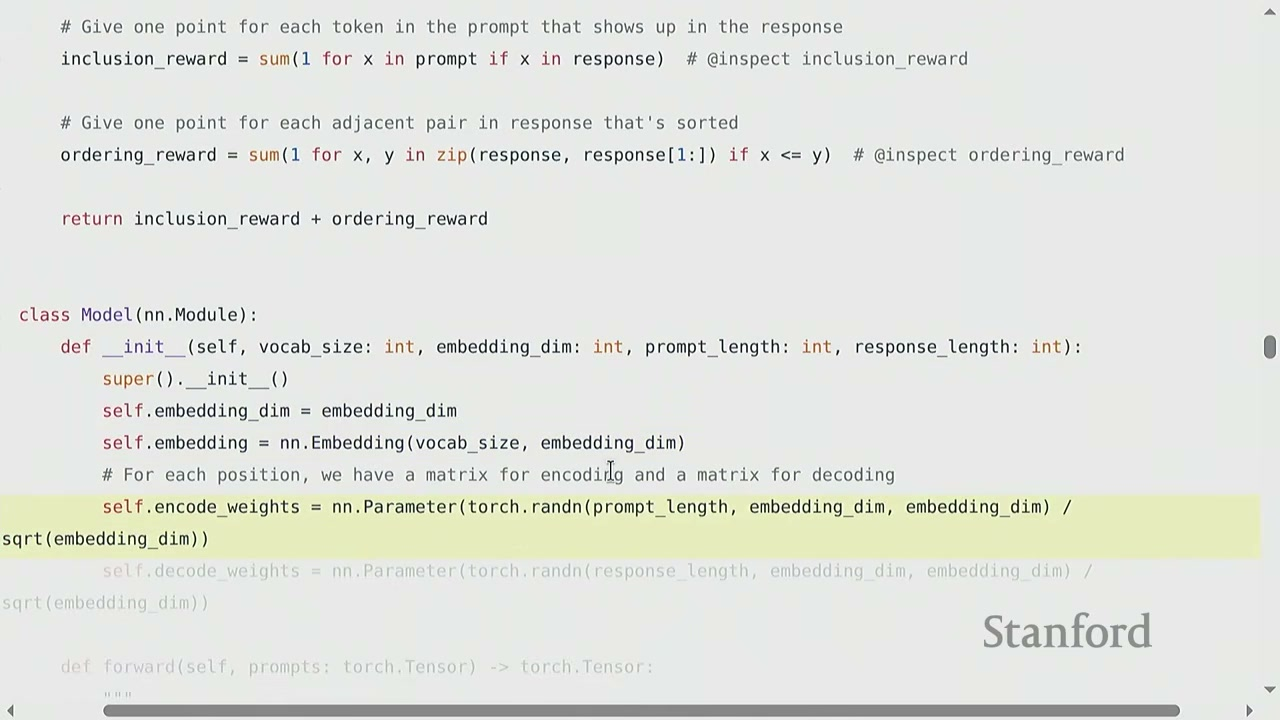
\includegraphics[width=\textwidth]{figures/fig_18_model_arch.jpg}
\caption{极简模型：每位置独立的 encode/decode 矩阵；非自回归——各位置独立解码\protect\footnotemark}
\end{figure}
\footnotetext{视频画面时间区间：00:38:30--00:39:15。}

为了让代码干净，Percy 设计了一个\textbf{非自回归}的极简模型（真实 LM 是自回归的，这里简化）：

\begin{itemize}
\item 假设 prompt 和响应长度固定且相等（都为 $n$）。
\item 用\textbf{每位置独立}的参数捕获位置信息（排序里位置是核心）。
\item \textbf{独立解码每个位置}：先编码整个序列，再对每个位置输出 token 分布（不是逐 token 自回归生成）。
\end{itemize}

\begin{knowledgebox}{为什么要偏离自回归？}
Percy 坦言：自回归生成那段代码"非常 hairy"，为了让讲解清晰他做了简化。这种"独立解码"在真实场景只在 speculative decoding 等少数地方有限使用，一般不这么做。但作为教学载体，它把注意力引向 RL 机制本身而非生成工程。
\end{knowledgebox}

模型组件：一个 embedding 矩阵；每个位置一个 encode 矩阵（$d_1 \to d_2$）和一个 decode 矩阵；最后映射到 vocab logits。

\subsection{前向与采样}

\begin{figure}[H]
\centering
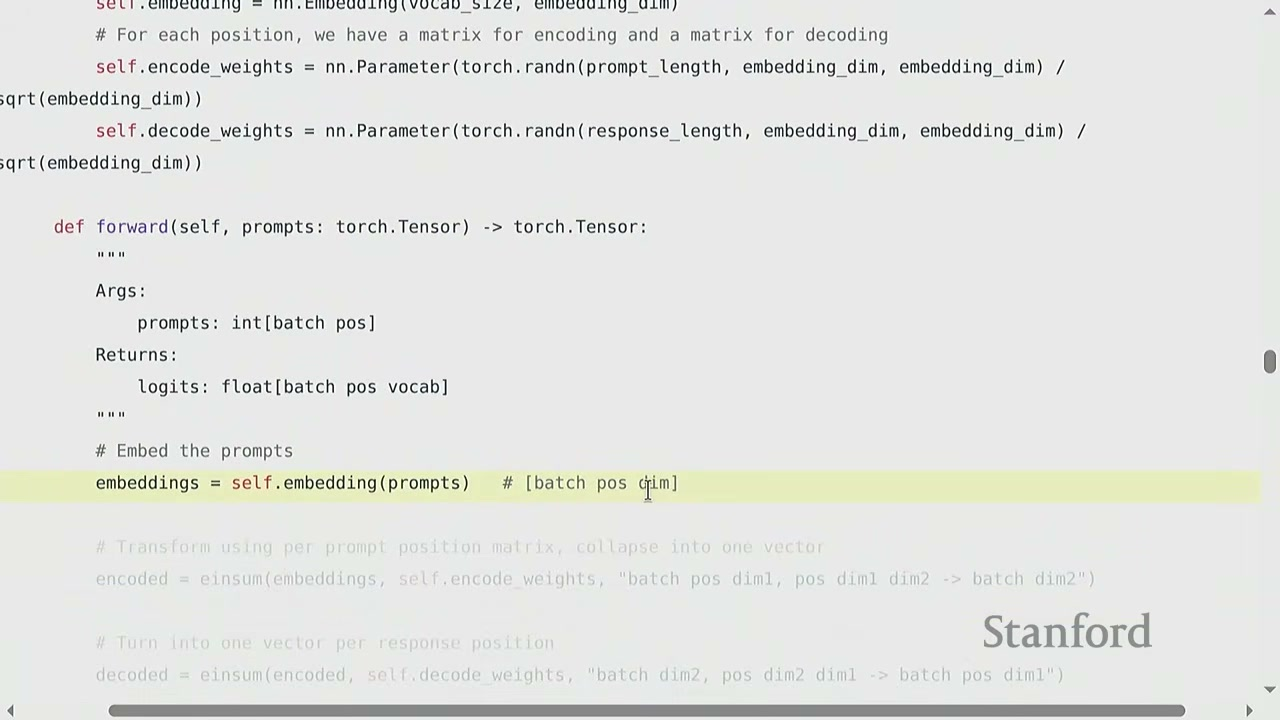
\includegraphics[width=\textwidth]{figures/fig_19_forward_pass.jpg}
\caption{推理流程：embed prompt $\to$ 逐位置变换 $\to$ logits $\to$ 采样 $G$ 条响应；维度 (batch, pos, trial)\protect\footnotemark}
\end{figure}
\footnotetext{视频画面时间区间：00:40:00--00:40:45。}

推理（生成 rollout）的维度流：

\begin{enumerate}
\item prompt 形状 $(B, n)$，$B$ 为 batch（prompt 数）。
\item embed 到 $(B, n, d_1)$，经每位置 encode 矩阵并按位置求和塌缩到 $(B, d_2)$。
\item 再对每位置用 decode 矩阵回到 $(B, n, d_2)$，最后映到 logits $(B, n, V)$，$V$ 为 vocab。
\item 把 logits 展平，对每 (batch, pos) 采样 $G$ 条 $\to$ 响应 $(B, n, G)$，重排为 $(B, G, n)$。
\end{enumerate}

\[
\text{logits}: (B, n, V) \;\xrightarrow{\text{sample }G}\; \text{resp}: (B, G, n)
\]

\begin{importantbox}{为什么响应"很接近"}
因为同一 (batch,pos) 的 $G$ 条响应都从同一 logits 分布独立采样，自然相似。这和真实 LM 从同分布多次采样同理，唯一区别是真实 LM 自回归、本模型独立。Percy 本想改温度引入更多 reward 方差，但为忠实于算法保持原样。
\end{importantbox}

\section{Delta、Log-prob 与损失}

\subsection{计算 delta：算法菜单}

\begin{figure}[H]
\centering
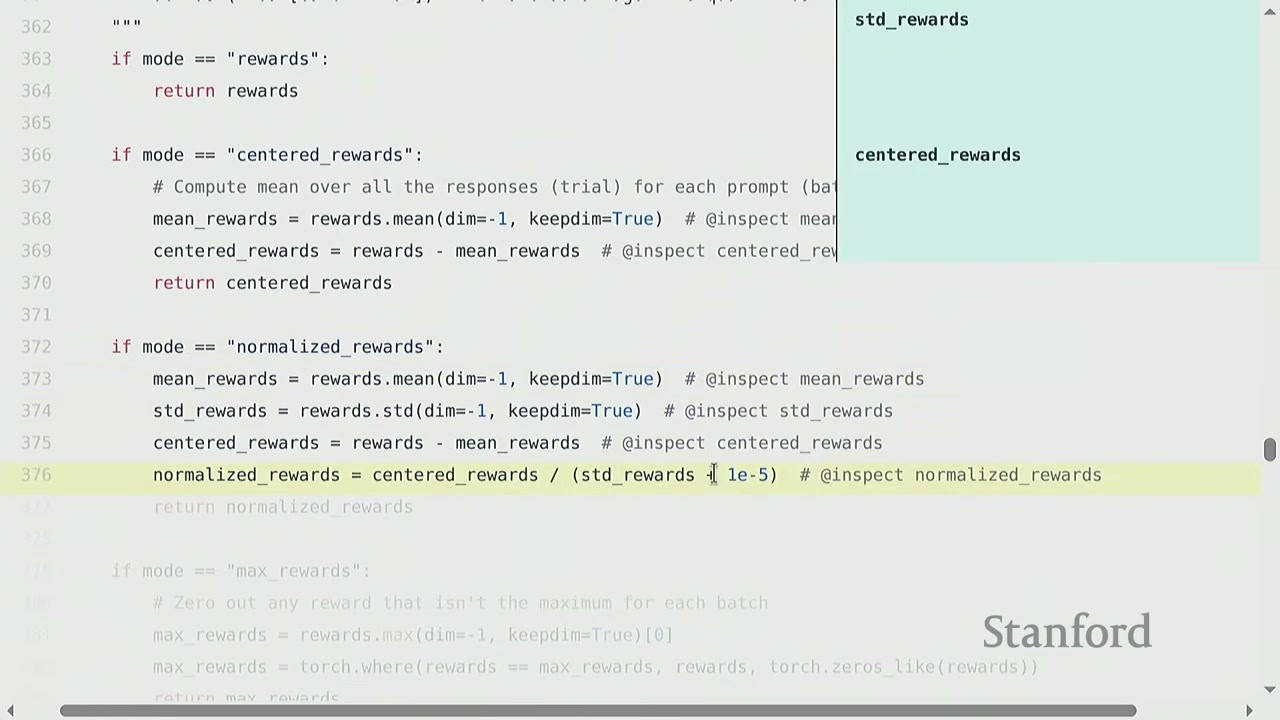
\includegraphics[width=\textwidth]{figures/fig_20_compute_deltas.jpg}
\caption{compute\_deltas 函数：原始 reward / 中心化（减均值）/ GRPO 标准化（再除标准差）/ 只保留最大值\protect\footnotemark}
\end{figure}
\footnotetext{视频画面时间区间：00:45:15--00:46:00。}

\texttt{compute\_deltas(rewards)} 把 reward 转成 $\delta$。Percy 把它呈现为一份"菜单"，对应 Assignment 5 学生要探索的选择：

\begin{enumerate}
\item \textbf{原始}：$\delta = r$（朴素策略梯度）。
\item \textbf{中心化}（centered）：每个 prompt 组内减均值。
\[
\delta_{i,g} = r_{i,g} - \frac{1}{G}\sum_{g'} r_{i,g'}
\]
回答了之前的提问：若 reward 是 $\{1,0,0,\ldots\}$，均值约 $0.1$，减去后错答得到负 $\delta$，于是也会被"推远"。
\item \textbf{GRPO 标准化}（normalized）：中心化后再除标准差（加小 $\epsilon$ 防除零）。
\[
\delta_{i,g} = \frac{r_{i,g} - \bar r_i}{\sigma_i + \epsilon}
\]
\item \textbf{只保留最大}（bonus）：把非组内最大的 reward 置零——"全有或全无"，对抗部分信用导致的局部最优。
\end{enumerate}

\begin{warningbox}{两个关键性质}
\begin{itemize}
\item \textbf{全相同则不更新}：若组内 reward 全是 5，中心化后 $\delta$ 全 0，不更新。直觉：组内没有相对差异，无法判断该偏爱谁，于是\textbf{弃权}，等别的样本给信号。
\item \textbf{尺度不变}：标准化后 reward 整体乘 100 不改变 $\delta$——对奖励的绝对尺度不敏感，这是 GRPO 的优良性质。
\end{itemize}
\end{warningbox}

\subsection{计算 log-prob}

\begin{figure}[H]
\centering
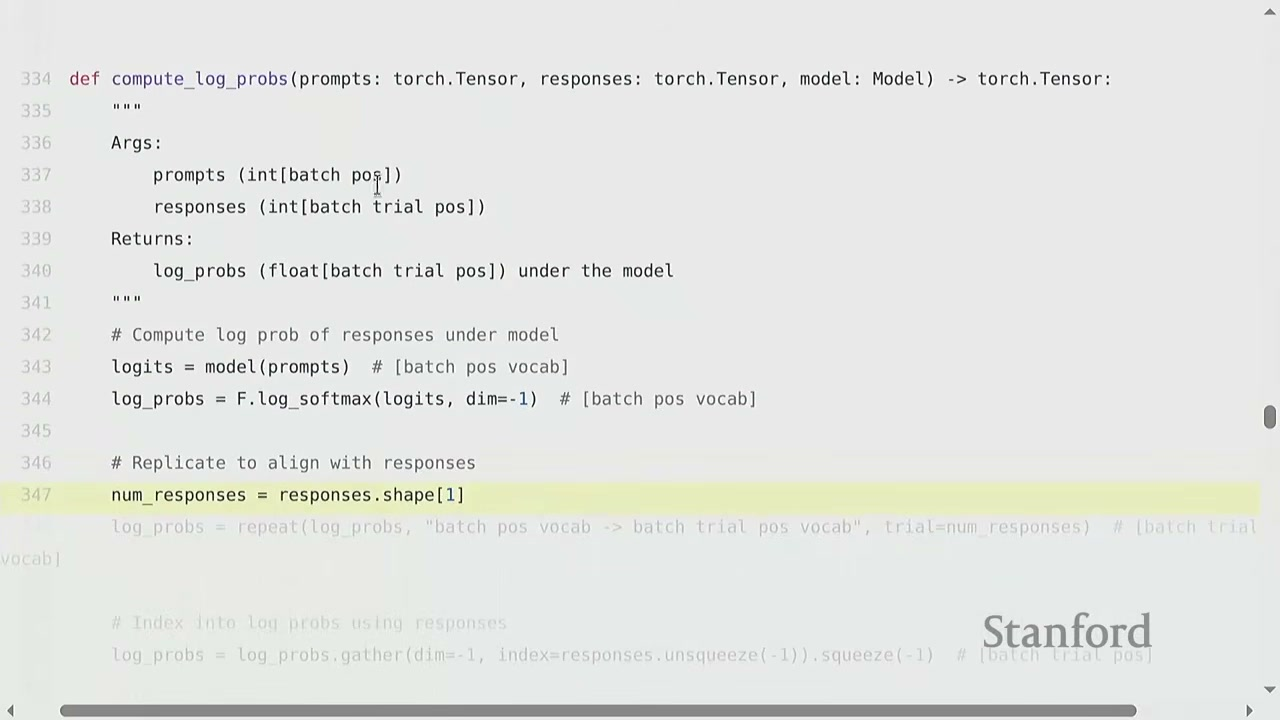
\includegraphics[width=\textwidth]{figures/fig_21_log_probs.jpg}
\caption{log-prob 计算：把响应过模型取 logits $\to$ log-softmax $\to$ 按响应 token 索引取出；形状 (batch, trial, pos)\protect\footnotemark}
\end{figure}
\footnotetext{视频画面时间区间：00:48:15--00:49:00。}

策略梯度还需要 $\nabla \log \pi$，所以要先拿到每条响应的对数概率：

\begin{enumerate}
\item 响应过模型 $\to$ logits $(B, G, n, V)$。
\item log-softmax 得到 log-prob。
\item 用响应张量作为索引，从 log-prob 中 gather 出每个实际 token 的对数概率 $\to (B, G, n)$。
\end{enumerate}

\[
\log \pi_\theta(\text{resp}) = \sum_{t=1}^{n} \log p_\theta(\text{resp}_t \mid \cdots)
\]

因为 outcome reward 的 $\delta$ 不依赖位置，它会被广播到每个位置；若用 process reward，$\delta$ 也会逐位置。

\subsection{no\_grad 插曲：冻结的艺术}

\begin{figure}[H]
\centering
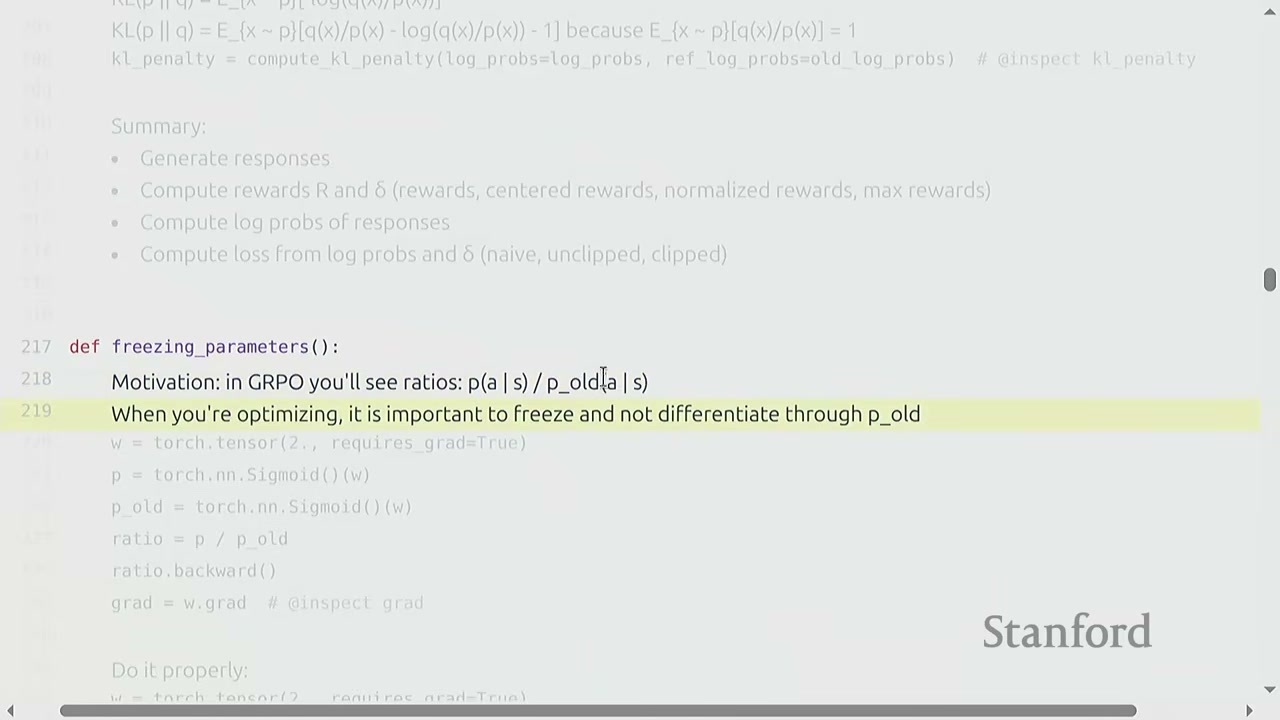
\includegraphics[width=\textwidth]{figures/fig_22_no_grad.jpg}
\caption{no\_grad 插曲：除以 $p_{\text{old}}$ 时若不冻结，比值恒为 1、梯度为 0；必须用 torch.no\_grad() 隔离计算图\protect\footnotemark}
\end{figure}
\footnotetext{视频画面时间区间：00:50:45--00:51:30。}

PPO/GRPO 里到处是"概率比" $\pi_\theta / \pi_{\text{old}}$。这里有个致命陷阱。设单参数 $w$ 同时驱动 $p$ 和 $p_{\text{old}}$：

\[
\text{ratio} = \frac{p(w)}{p_{\text{old}}(w)} = 1 \quad\Longrightarrow\quad \nabla_w 1 = 0
\]

\begin{warningbox}{常见 bug：梯度全为零}
若 $p_{\text{old}}$ 也参与计算图，比值求导恒为零，模型完全不学。\textbf{必须}用 \texttt{torch.no\_grad()} 把任何要当常数的量包起来——拿到数值但切断梯度。RL 与预训练的关键区别：RL 里同时存在"新参数"和"旧/冻结参数"，要时刻清楚谁在计算图里。
\end{warningbox}

\subsection{GRPO 的 clipped loss}

\begin{figure}[H]
\centering
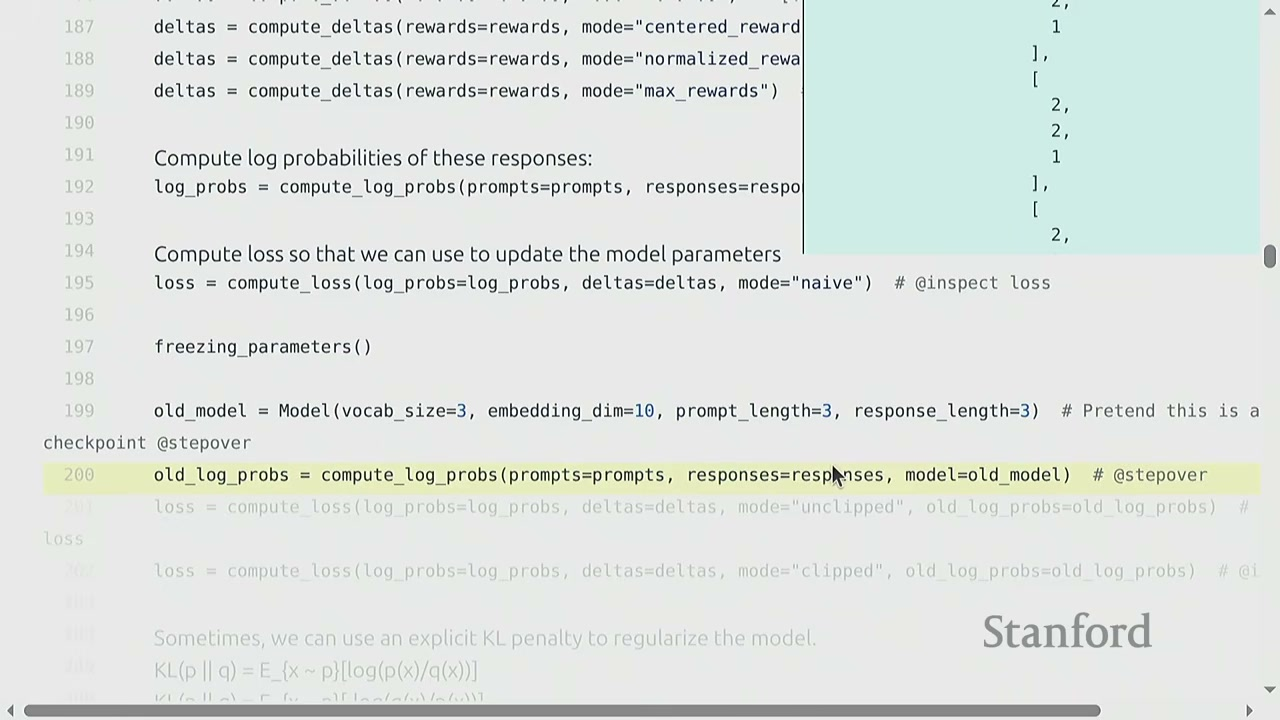
\includegraphics[width=\textwidth]{figures/fig_23_grpo_loss.jpg}
\caption{GRPO 损失：ratio $\cdot \delta$ 与 clip(ratio)$\cdot\delta$ 取 min，再加负号变 loss；clip 把更新幅度限制在 $[1-\epsilon, 1+\epsilon]$\protect\footnotemark}
\end{figure}
\footnotetext{视频画面时间区间：00:53:45--00:54:30。}

GRPO 损失（clip 版）：

\[
\mathcal{L}_{\text{GRPO}} = -\mathbb{E}\left[ \min\left( \rho\,\delta,\; \text{clip}(\rho, 1-\epsilon, 1+\epsilon)\,\delta \right) \right]
\]

其中 $\rho = \pi_\theta(a\mid s) / \pi_{\text{old}}(a\mid s) = \exp(\log\pi_\theta - \log\pi_{\text{old}})$。

\begin{importantbox}{clip 的作用}
\begin{itemize}
\item 若 ratio $\rho$ 落在 $[1-\epsilon, 1+\epsilon]$ 内，clip 不生效，等价于朴素策略梯度（只是多除了个常数 $p_{\text{old}}$，相当于缩放梯度）。
\item 若 $\rho$ 超出范围，更新幅度被夹在 $[1-\epsilon, 1+\epsilon]$ 乘 $\delta$。\textbf{目的}：防止策略在单步内偏离 old 策略太远，保持训练稳定。
\item 取 min 是 PPO 的标准技巧（trust region 思想）；外层加负号是因为把"最大化 reward"翻成"最小化 loss"。
\end{itemize}
\end{importantbox}

\subsection{KL 惩罚：低方差估计}

\begin{figure}[H]
\centering
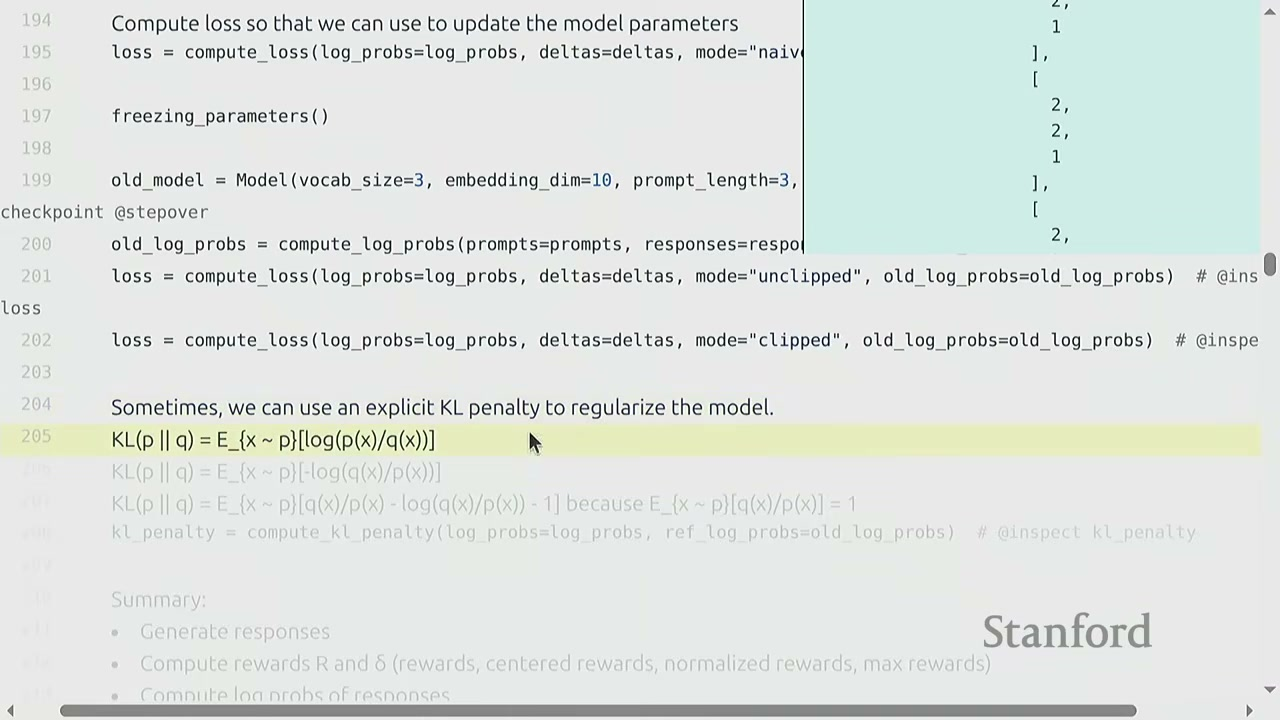
\includegraphics[width=\textwidth]{figures/fig_24_kl_penalty.jpg}
\caption{KL 惩罚推导：$D_{\text{KL}}(q\|p) = \mathbb{E}_q[\log(q/p)]$；用 $q/p - \log(q/p) - 1$ 得到同期望但更低方差的无偏估计\protect\footnotemark}
\end{figure}
\footnotetext{视频画面时间区间：00:56:15--00:57:00。}

GRPO 常加一个 KL 正则，把策略拉向参考模型 $\pi_{\text{ref}}$（防漂移/防 reward hacking）。KL 散度定义：

\[
D_{\text{KL}}(q \,\|\, p) = \mathbb{E}_{x \sim q}\left[ \log \frac{q(x)}{p(x)} \right]
\]

朴素无偏估计是直接采样求 $\log(q/p)$ 的均值。但有个\textbf{更低方差}的等价形式：

\[
\hat{D}_{\text{KL}} = \mathbb{E}_{x \sim q}\left[ \frac{q(x)}{p(x)} - \log\frac{q(x)}{p(x)} - 1 \right]
\]

\begin{knowledgebox}{为什么等价？}
因为 $\mathbb{E}_{x \sim q}[q(x)/p(x)] = \int q \cdot \frac{q}{p}\,dx$……这里的关键是 $\mathbb{E}_{q}[q/p]$ 这一项按重写后等于常数 1（在理想情况下），减 1 抵消，剩下的就是原始 KL。而把 $q/p$ 这一项塞进来降低了估计方差。\textbf{这是 RL 的常见手艺}：把估计式重写成期望相同但方差更低的形式（控制变量/control variate 的思想）。
\end{knowledgebox}

实现上，KL 惩罚在 vocab 维度求和、在 (batch, trial, pos) 维度取均值。Percy 说实际中加不加"区别不大"，是个可选的正则项。

\section{完整训练循环}

\subsection{三层循环结构}

\begin{figure}[H]
\centering
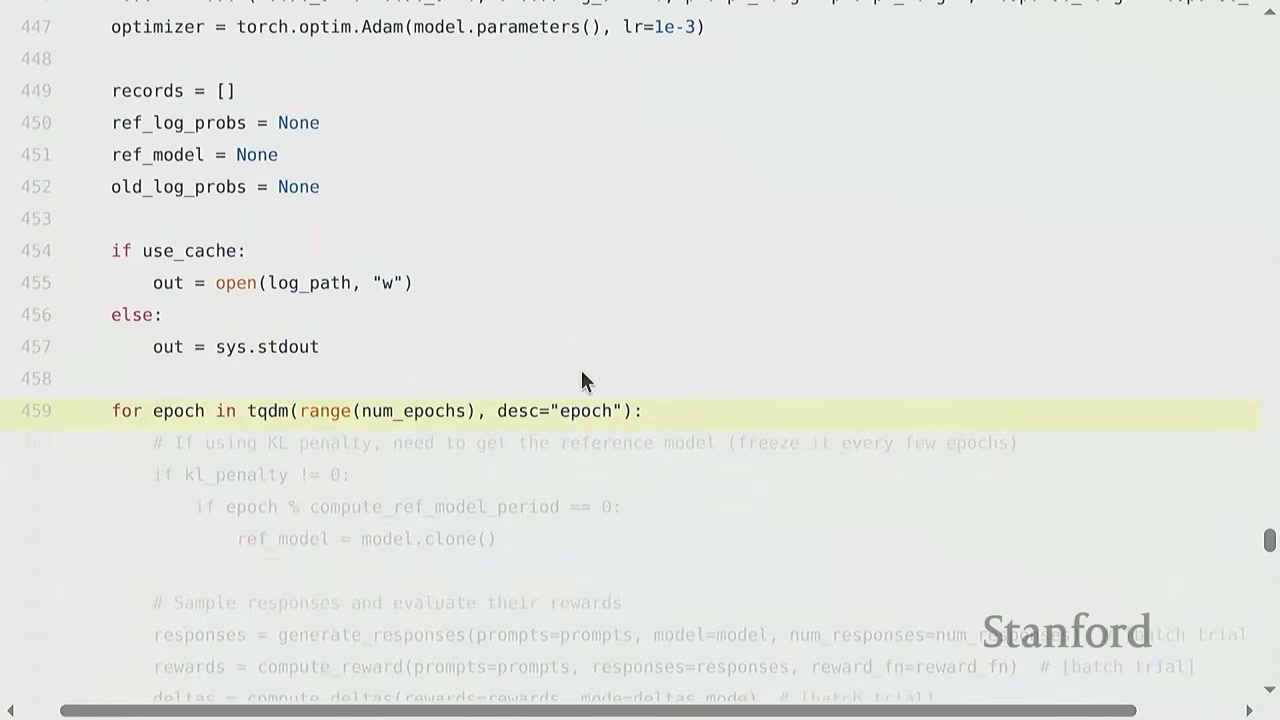
\includegraphics[width=\textwidth]{figures/fig_25_full_algorithm.jpg}
\caption{完整算法：外层 epoch 循环（更新 reference）$\to$ 采样响应 $\to$ 内层多步梯度更新；推理昂贵，故对同一批响应做多次更新\protect\footnotemark}
\end{figure}
\footnotetext{视频画面时间区间：01:00:15--01:01:00。}

把所有组件拼起来，GRPO 训练循环的骨架：

\begin{lstlisting}[language=Python]
model = SimpleModel(...); opt = AdamW(model.parameters())
ref_model = copy(model)   # reference / anchor, updated slower
for epoch in range(E):
    # if using KL penalty, freeze a reference copy first
    ref_model = maybe_update_ref(model, ref_model)
    for prompts in dataloader:
        # 1) rollout generation (inference, expensive)
        responses = model.generate(prompts, num_responses=G)
        # 2) reward + delta (model-independent)
        rewards = reward_fn(prompts, responses)
        deltas = compute_deltas(rewards)         # raw/centered/normalized
        # 3) old policy log-prob (frozen, for ratio)
        with torch.no_grad():
            old_logp = model.log_prob(responses)
        # 4) inner loop: multiple updates on same responses
        for step in range(inner_steps):
            logp = model.log_prob(responses)
            loss = grpo_loss(logp, old_logp, deltas, eps) \
                   + beta * kl_penalty(model, ref_model, responses)
            opt.step(loss.backward())
\end{lstlisting}

\begin{importantbox}{为什么有内层循环？}
\textbf{推理（rollout）非常昂贵}，所以拿到一批响应后要多走几个梯度步榨干它的价值。这就是双层循环的动机：外层重新采样，内层多次更新。若加 KL，还多一个\textbf{最外层}更新参考模型的循环（reference 比 policy 更新更慢）。
\end{importantbox}

\subsection{参考模型与"慢节奏"}

\begin{figure}[H]
\centering
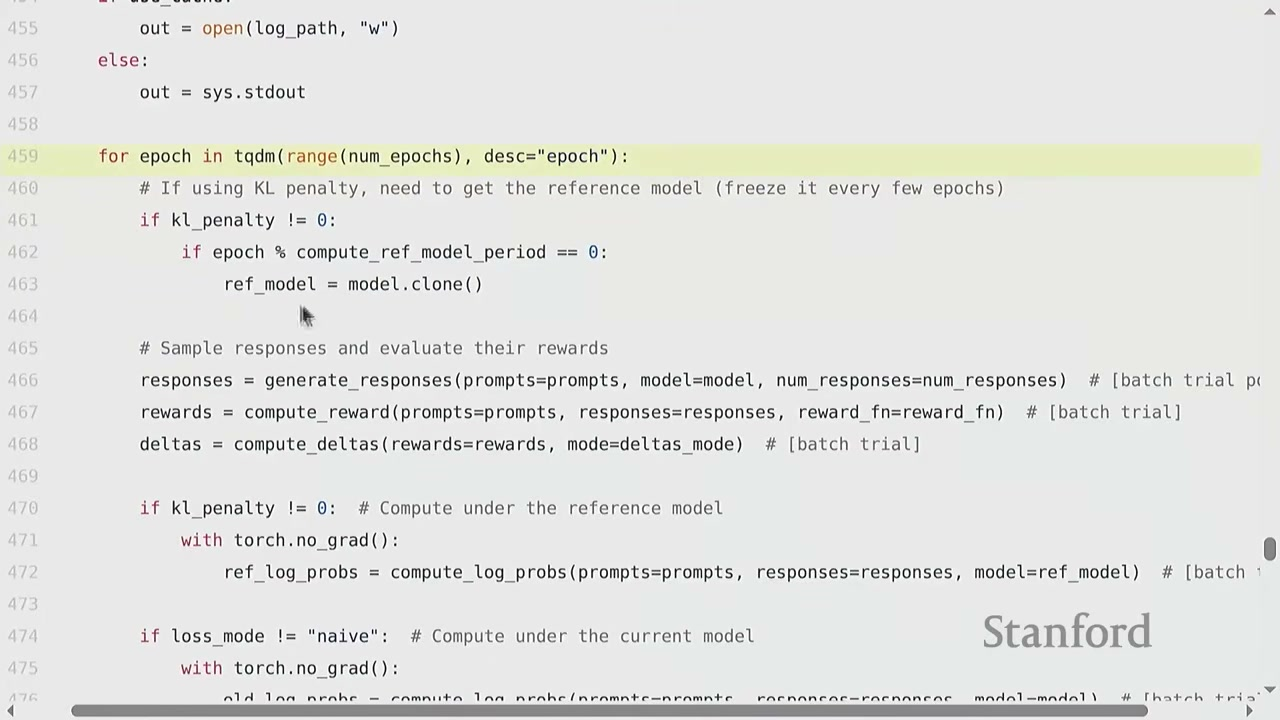
\includegraphics[width=\textwidth]{figures/fig_26_big_picture.jpg}
\caption{大局：外层生成 rollout + 内层多次更新；KL 惩罚则引入比策略更新更慢的参考模型作为锚点\protect\footnotemark}
\end{figure}
\footnotetext{视频画面时间区间：01:02:30--01:03:15。}

\begin{warningbox}{三层"时间尺度"}
GRPO 的完整图景包含三个不同节奏：
\begin{itemize}
\item \textbf{响应采样}（最慢、最贵）：固定模型，采样一批 rollout。
\item \textbf{策略更新}（中速）：对这批 rollout 走 inner\_steps 步梯度。
\item \textbf{参考模型}（最慢更新）：KL 惩罚锚定的 $\pi_{\text{ref}}$，更新频率比策略还低。
\end{itemize}
Percy 的代码版为了简洁把 reference 更新得"有点频繁"，与官方 GRPO 实现的"三循环"略有出入，但教学上已足够。
\end{warningbox}

\section{Assignment 5 与延伸}

\subsection{与作业的对应}

本讲整个"算法菜单"正是 Assignment 5 的探索空间。学生要在真实（或半真实）的 LM 上实现 RL，并比较不同 $\delta$ 变体、clip 与否、KL 与否的效果。

\begin{practicebox}{A5 的关键决策点}
\begin{itemize}
\item \textbf{$\delta$ 选择}：原始 / 中心化 / GRPO 标准化 / 只保留最大——不同选择影响收敛速度与最终性能。
\item \textbf{clip}：开/关，$\epsilon$ 取值——稳定性与学习速度的权衡。
\item \textbf{KL 惩罚}：开/关，$\beta$ 取值——是否需要锚定参考模型。
\item \textbf{奖励设计}：稀疏 0/1 还是部分信用——直接决定能否逃出冷启动陷阱。
\item \textbf{工程细节}：\texttt{no\_grad} 包裹旧/参考量、gather log-prob、维度对齐。
\end{itemize}
\end{practicebox}

\subsection{过程奖励与多轮交互}

Percy 在问答中补充了两个方向：

\begin{itemize}
\item \textbf{过程奖励（process reward）}：outcome reward 只在结尾给信号；若能在中间步骤评估（如每步推理是否正确），梯度会更稠密、方差更低。但 LM 的过程奖励\textbf{极难做好}——除非明显跑偏，否则很难判断中间步骤的好坏。
\item \textbf{尽早评估}：如果有可信的中间信号，应尽早评估 reward。
\end{itemize}

关于折扣（discounting）：有人问"是否该给结尾 token 更大权重"。Percy 认为不明确——早期决策往往更重要（选对策略后续自然展开），而 RL 的难处正在于\textbf{不知道信用该分配给谁}，所以这里把信用"均匀涂抹"在整条轨迹上。

\subsection{本讲小结}

\begin{importantbox}{核心要点回顾}
\begin{enumerate}
\item \textbf{设置}：语言模型 RL 的状态是 token 序列，动作是下一 token，转移动力学是简单拼接——这使规划（test-time compute）成为可能，状态可被模型"自由构造"。
\item \textbf{策略梯度}：$\nabla J \approx \nabla\log\pi \cdot \delta$ 是永恒框架；$\delta$ 的具体形式（reward/中心化/标准化）对应不同算法。
\item \textbf{基线与优势}：减去只依赖状态的基线不改变期望梯度但降方差；选 $B(s)=V(s)$ 时 advantage 凸显"比平均好多少"。
\item \textbf{GRPO}：利用"一 prompt 多采样"的天然分组估计 $V(s)$ 和 $\sigma(s)$，免去 value function；clip 稳定训练，KL 惩罚锚定参考模型。
\item \textbf{工程纪律}：旧/参考量必须 \texttt{no\_grad}；推理昂贵故用内层多步更新；reward 设计要给部分信用以对抗稀疏陷阱。
\end{enumerate}
\end{importantbox}

\subsection{配套阅读}

\begin{tabular}{p{7cm}p{6cm}}
\toprule
\textbf{材料} & \textbf{对应知识点} \\
\midrule
PPO: Schulman et al. 2017 & clip ratio、trust region \\
GRPO: DeepSeek 2024 & 组内标准化、去 value function \\
Chelsea Finn: CS285 Deep RL & 策略梯度与基线的完整推导 \\
Assignment 5 (CS336) & 本讲代码的实战实现 \\
\bottomrule
\end{tabular}

%% --- 正文内容结束 ---

\end{document}
